
\documentclass[twoside,11pt]{article}

\usepackage[T1]{fontenc}
\IfFileExists{lmodern.sty}{\usepackage{lmodern}}{}
\usepackage[preprint]{jmlr2e}

\usepackage{amsmath,amssymb,amsfonts,bm,mathtools}
\usepackage{booktabs,array,tabularx}
\usepackage{algorithm}
\usepackage{algpseudocode}
\usepackage{enumitem}
\usepackage{lastpage}
\IfFileExists{xurl.sty}{\usepackage{xurl}}{\usepackage{url}}
\urlstyle{tt}
\setlength{\textfloatsep}{10pt plus 2pt minus 2pt}
\setlength{\floatsep}{8pt plus 2pt minus 2pt}
\setlength{\intextsep}{8pt plus 2pt minus 2pt}
\renewcommand{\topfraction}{0.90}
\renewcommand{\bottomfraction}{0.80}
\renewcommand{\textfraction}{0.08}
\renewcommand{\floatpagefraction}{0.80}
\setlength{\abovecaptionskip}{4pt}
\setlength{\belowcaptionskip}{0pt}
\setlength{\abovedisplayskip}{6pt plus 2pt minus 3pt}
\setlength{\belowdisplayskip}{6pt plus 2pt minus 3pt}
\setlength{\abovedisplayshortskip}{3pt plus 2pt minus 2pt}
\setlength{\belowdisplayshortskip}{4pt plus 2pt minus 2pt}
\allowdisplaybreaks[1]
\raggedbottom

\makeatletter
\setlength{\@fptop}{0pt}
\setlength{\@fpsep}{12pt plus 4pt}
\setlength{\@fpbot}{0pt plus 1fil}
\makeatother

\makeatletter
\let\lemma\relax
\let\endlemma\relax
\let\thelemma\relax
\let\proposition\relax
\let\endproposition\relax
\let\theproposition\relax
\let\remark\relax
\let\endremark\relax
\let\theremark\relax
\let\corollary\relax
\let\endcorollary\relax
\let\thecorollary\relax
\let\definition\relax
\let\enddefinition\relax
\let\thedefinition\relax
\let\conjecture\relax
\let\endconjecture\relax
\let\theconjecture\relax
\let\axiom\relax
\let\endaxiom\relax
\let\theaxiom\relax
\makeatother
\newtheorem{lemma}{Lemma}
\newtheorem{proposition}{Proposition}
\newtheorem{remark}{Remark}
\newtheorem{corollary}{Corollary}
\newtheorem{definition}{Definition}
\newtheorem{conjecture}{Conjecture}
\newtheorem{axiom}{Axiom}
\newtheorem{assumption}{Assumption}

\newcommand{\D}{\mathcal{D}}
\newcommand{\F}{\mathcal{F}}
\newcommand{\Fp}{\mathfrak{F}}
\newcommand{\G}{\Gamma}
\newcommand{\E}{\mathbb{E}}
\newcommand{\PP}{\mathbb{P}}
\newcommand{\R}{\mathbb{R}}
\newcommand{\ind}{\mathbf{1}}
\newcommand{\TV}{\operatorname{TV}}
\newcommand{\KL}{\operatorname{KL}}
\newcommand{\tr}{\operatorname{tr}}
\newcommand{\rank}{\operatorname{rank}}
\newcommand{\supp}{\operatorname{supp}}

\jmlrheading{0}{2026}{1-\pageref{LastPage}}{}{}{preprint}{Hanqing Li, Xuewen Lu, and Yuting Chen}
\ShortHeadings{Bayesian Model Averaging under Predictor Redundancy}{Li, Lu, and Chen}
\firstpageno{1}
\hypersetup{hypertexnames=false}
\AtBeginDocument{%
\providecommand*{\theHfigure}{\arabic{figure}}%
\providecommand*{\theHtable}{\arabic{table}}%
\providecommand*{\theHalgorithm}{\arabic{algorithm}}%
\renewcommand*{\theHfigure}{bmafig.\arabic{figure}}%
\renewcommand*{\theHtable}{bmatab.\arabic{table}}%
\renewcommand*{\theHalgorithm}{bmaalg.\arabic{algorithm}}%
}
\newif\ifBMAincludeSupplement
% The default review build includes the appendices. Switch to
% \BMAincludeSupplementfalse only when preparing a short main-paper copy.
\BMAincludeSupplementtrue

\begin{document}

\title{Bayesian Model Averaging under Predictor Redundancy}

\author{\name Hanqing Li \email hanqing.li@ucalgary.ca \\
       \addr Department of Mathematics and Statistics\\
University of Calgary\\ Calgary, AB T2N 1N4, Canada
       \AND
       \name Xuewen Lu \email xlu@ucalgary.ca \\
       \addr Department of Mathematics and Statistics\\
University of Calgary\\ Calgary, AB T2N 1N4, Canada
       \AND
       \name Yuting Chen \email yuting.chen@eku.edu \\
       \addr Department of Mathematics and Statistics\\
Eastern Kentucky University\\ Richmond, KY 40475, USA}

\maketitle

\begin{abstract}
Bayesian model averaging can spread posterior mass over many nearly interchangeable model supports. The stable scientific message may be a region of support space rather than one exact support. We study density-ratio posterior compression for a fixed unrestricted support posterior. A support kernel \(w:\Gamma_p\to[0,1]\) is a weight function for a hard or soft support-space region. Normalizing the posterior after multiplying by \(w\) gives a restricted posterior component, and mixtures of these components have an exact density ratio \(h_q\) relative to the unrestricted posterior. This ratio gives total variation, forward and reverse KL, predictive contraction, and fallback diagnostics for many summaries of the same posterior. The construction covers fixed hard regions, structured kernels, posterior-cluster kernels, pooled-pruned hybrids, and top-\(M\) atoms. We prove iid and blocked-MCMC validation bounds, candidate-pool coverage results, structural redundancy examples, and an atom-region separation showing when top-\(M\) atom storage is inefficient. The experiments use Gaussian linear BMA for exact and large-\(p\) benchmarks, report \(q_0\)-screened frontiers to separate region compression from fallback use, and include a small logistic support-posterior algebra check after exact support enumeration. The method is a posterior reporting and validation layer, not a replacement for reference-posterior computation.
\end{abstract}

\begin{keywords} Bayesian model averaging, density-ratio posterior compression, support kernels, predictor redundancy, model uncertainty
\end{keywords}

\section{Introduction}

Bayesian model averaging (BMA) averages over supports instead of conditioning on a single selected model \citep{hoeting1999,forte2018}. This protects model uncertainty, but predictor redundancy creates a summarization problem that subset averaging alone does not solve. The problem occurs both in classical regimes with moderate \(p\) and in high-dimensional sparse regimes where \(p\) may be comparable to or larger than \(n\). A posterior can concentrate on simple models while spreading its mass over many near-substitute supports. The support posterior is discrete, so one exact support \(\gamma\) with positive posterior mass is an atom of the posterior measure. The scientifically stable object may then be a region of support space, rather than any particular atom.

This paper treats that situation as a posterior-compression problem for a fixed unrestricted support posterior. We seek low-complexity hard or soft support-space regions that preserve enough of the unrestricted posterior to be reported with quantitative distortion diagnostics. The practical regimes are easiest to see as recurring redundancy patterns rather than as one application. Figure~\ref{fig:practicalregimes} sketches three common cases.
\begin{itemize}[leftmargin=1.8em,itemsep=1pt,topsep=3pt]
\item \textbf{Spectroscopy.} Adjacent wavelength channels can measure the same broad absorption feature, so many posterior-plausible supports differ only by which nearby channel is chosen.
\item \textbf{Molecular modules.} Co-expressed probes or genes can act as substitutes for the same biological module. The module-level posterior message may be stable even when the exact probe is not.
\item \textbf{Spatial, sensor, and lagged designs.} Neighboring sensors, nearby locations, climate covariates, or adjacent lags can encode the same effect, making the relevant region or window more interpretable than one selected coordinate.
\end{itemize}
In all three cases, the goal is not to identify a uniquely correct representative, but to report posterior model uncertainty at the resolution at which the predictors are interpretable.

\begin{figure}[!htbp]
\centering
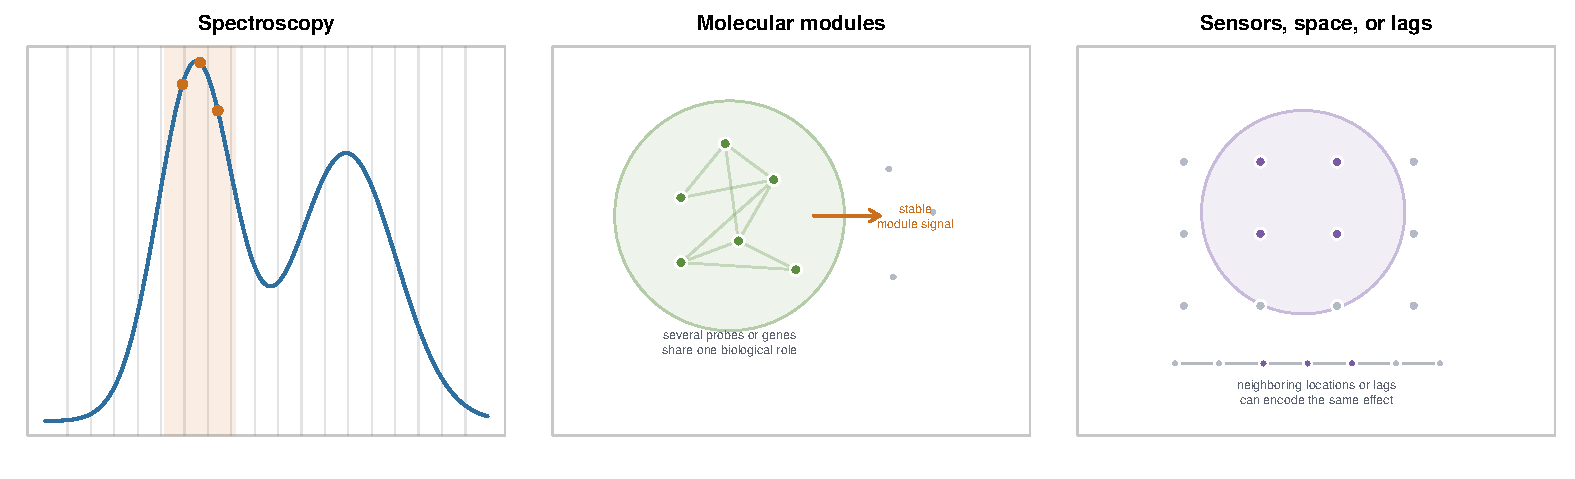
\includegraphics[width=\textwidth]{sim/output/practical_regime_examples.pdf}
\caption{Predictor redundancy regimes motivating support-space summaries. Left to right, the panels show spectroscopy, molecular modules, and spatial, sensor, or lagged designs.}
\label{fig:practicalregimes}
\end{figure}

The closest neighboring ideas are ordinary BMA model lists, posterior clustering or block summaries under collinearity, and dilution or powered-correlation priors. Top-\(M\) BMA lists keep the largest support atoms and are the natural atom-level baseline \citep{hoeting1999,clyde2011}. Posterior clustering and block summaries organize fitted posterior samples, but they usually report clusters without an exact distortion check against the original posterior \citep{ghosh2015collinearity,papaspiliopoulos2017}. Dilution and powered-correlation priors address redundancy before fitting by changing support prior weights, so they change the Bayesian target \citep{george2010,krishna2009}. Projection predictive methods and penalized regression methods mainly compress prediction or coefficients rather than the support posterior \citep{zou2005,yuan2006,simon2013,bair2006,piironen2017,piironen2020}.

Our target is different. We keep the unrestricted BMA posterior fixed and ask whether its support-space uncertainty can be reported at a coarser resolution with a quantitative distortion check. Table~\ref{tab:relatedwork} gives a short map of this landscape. Section~\ref{subsec:existingsummaries} turns the closest support-summary ideas into reusable templates.

The basic building block is a support kernel \(w:\Gamma_p\to[0,1]\). This is a weight function on model supports. A value near one means that the support is inside the region. A value near zero means that it is outside. Values between zero and one allow soft boundaries. A hard support region is the special case \(w(\gamma)=\ind\{\gamma\in\F\}\). Multiplying the unrestricted posterior by \(w\) and renormalizing gives the posterior restricted to that region. A mixture of several restricted posteriors is easy to check because it has an exact density ratio \(h_q\) relative to the unrestricted posterior. Once this ratio is known, total variation, forward and reverse KL, predictive contraction, retained kernel mass, and the fallback weight \(q_0\) become direct diagnostics rather than informal summaries.

This density-ratio view is the organizing idea of the paper. It does not prescribe one dictionary. Fixed hard regions, group-representative regions, interval kernels, graph kernels, residual-cover kernels, posterior-cluster kernels, pooled-pruned dictionaries, and top-\(M\) atom truncations can all be evaluated in the same units once they are written as support kernels. Group-representative regions are an important response-independent special case. Posterior-adaptive kernels, including cluster kernels learned from posterior support samples, are checked summaries of an already fitted reference posterior.

The empirical question follows from this view. We first ask whether density-ratio compression gives useful posterior-compression tradeoffs compared with methods that change the target or only predict. We then ask which dictionary family works best for a given reporting goal. Posterior-cluster kernels are one dictionary family inside the framework. Structured and pooled-pruned kernels are another, aimed at low expected code and interpretable region summaries. Top-\(M\) atoms are the atom-level limiting case. The paper is therefore a way to check posterior summaries on a common density-ratio scale, not a claim that one dictionary is uniformly best.

We use a few paper-specific terms. A support atom is one exact model support \(\gamma\). A support region is a set or soft neighborhood of atoms. A support kernel is the weight function used to describe such a region. A dictionary is the finite list of regions available to the compression. A code length is the storage cost of reporting a region. The fallback weight \(q_0\) is the mixture weight left on unrestricted BMA. A large \(q_0\) means that the learned regions did not explain much of the posterior by themselves. A held-out check means a theorem-backed density-ratio validation relative to the chosen reference posterior. It does not prove that the reference posterior sampler itself is correct.

The workflow starts from a trustworthy reference posterior on the unrestricted support space. The reference may come from exact enumeration, MCMC, SMC, variational approximation, or another model-specific Bayesian engine. At the compression stage, the density-ratio calculation does not require a Gaussian likelihood or a Gaussian coefficient prior. The reproducible experiments use a regularized Gaussian linear BMA instance because it gives exact small-\(p\) checks and stable large-\(p\) diagnostics. Candidate regions are learned on one posterior split. Their masses are estimated on a second split. Mixture weights are optimized on validation draws, and final distortion is reported on held-out draws. These splits matter because some dictionaries are learned from the posterior sample. The compression result is useful only when the reference posterior itself is trustworthy. Failed reference diagnostics make the compression exploratory rather than validated.

This scope is part of the method. The paper does not introduce a new prior, a new reference-posterior sampler, or a universal variable-selection rule. It gives a way to compress and check a fixed support posterior after that posterior has been computed. A reported summary is successful only when posterior distortion is small, expected descriptor cost is small, the active descriptor list is shown, and the fallback weight \(q_0\) is not carrying most of the approximation. We therefore report \(q_0\)-screened frontiers in the main large-\(p\) benchmark rather than relying on a single fitted point.

The paper has one organizing contribution, density-ratio posterior compression for a fixed support posterior. The formal work supports this idea in three pieces.
\begin{enumerate}[leftmargin=1.8em,itemsep=0.35em,topsep=0.35em,parsep=0pt,partopsep=0pt]
\item We define support-kernel compression and give exact density-ratio diagnostics. The same identity gives TV, forward KL, reverse KL, predictive contraction, and the fallback weight \(q_0\). Hard regions and retained mass are the simplest special case.
\item We give validation theory for learned dictionaries. The main guarantees are a held-out density-ratio check, a blocked-MCMC version, and a candidate-pool cover bound. Smaller supporting results explain how the conditions hold for clusters, group regions, and intervals.
\item We compare region summaries with atom summaries. The algorithm section turns several familiar summaries into density-ratio checked dictionaries. The atom-storage theorem explains why top-\(M\) support lists can be inefficient under representative redundancy.
\end{enumerate}

Figure~\ref{fig:compressionillustration} illustrates the target object in a small enumerable redundant example.

\enlargethispage{2\baselineskip}
\begin{figure}[H]
\centering
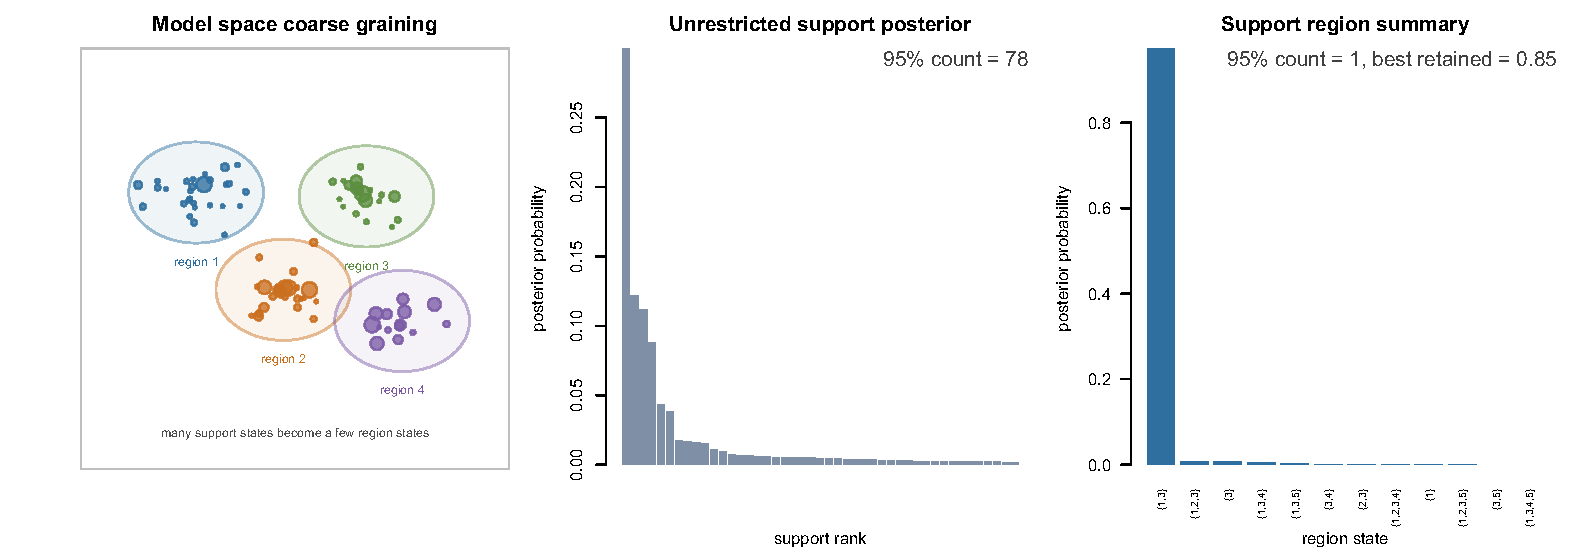
\includegraphics[width=\textwidth]{sim/output/model_space_compression_illustration.pdf}
\caption{Support-kernel compression in an enumerable redundant example. Many atom-level supports are reported as a few support regions, with the density-ratio check measuring the information lost.}
\label{fig:compressionillustration}
\end{figure}
\vspace{8\baselineskip}

Table~\ref{tab:relatedwork} is meant as a scan table rather than a second literature review. The empirical section uses it in two ways. It compares the proposed density-ratio summaries with outside methods that change the target or focus on prediction, and it compares dictionary families inside the framework on the same posterior-distortion scale.

\begin{table}[!htbp]
\centering
\scriptsize
\setlength{\tabcolsep}{3.0pt}
\renewcommand{\tabularxcolumn}[1]{m{#1}}
\setlength{\extrarowheight}{0pt}
\renewcommand{\arraystretch}{1.0}
\begin{tabularx}{0.985\textwidth}{@{}>{\raggedright\arraybackslash}m{0.23\textwidth}
>{\raggedright\arraybackslash}m{0.115\textwidth}
>{\raggedright\arraybackslash}m{0.13\textwidth}
>{\raggedright\arraybackslash}m{0.13\textwidth}
>{\raggedright\arraybackslash}X@{}}
\toprule
method class & object & redundancy handling & output & role here \\
\midrule
\end{tabularx}
\vspace{-0.25em}
\setlength{\extrarowheight}{1.0pt}
\renewcommand{\arraystretch}{1.30}
\begin{tabularx}{0.985\textwidth}{@{}>{\raggedright\arraybackslash}m{0.23\textwidth}
>{\raggedright\arraybackslash}m{0.115\textwidth}
>{\raggedright\arraybackslash}m{0.13\textwidth}
>{\raggedright\arraybackslash}m{0.13\textwidth}
>{\raggedright\arraybackslash}X@{}}
\rule[-0.85ex]{0pt}{3.7ex}Unrestricted support level BMA and stochastic search
& individual supports
& sparsity prior
& support posterior
& reference target and atom-list baseline \\
\rule[-0.85ex]{0pt}{3.7ex}Structured support MCMC, SMC, and variational BMA
& posterior engine
& improves exploration
& samples or approximate law
& possible source of the reference posterior \\
\rule[-0.85ex]{0pt}{3.7ex}Dilution and powered correlation priors
& support prior mass
& downweights crowding
& modified posterior
& outside Bayesian baseline because the target changes \\
\rule[-0.85ex]{0pt}{3.7ex}Determinantal priors
& support configurations
& repulsive prior
& modified posterior
& outside Bayesian baseline because the target changes \\
\rule[-0.85ex]{0pt}{3.7ex}Group spike and slab priors
& group inclusion
& prespecified group sparsity
& coefficient or group posterior
& Bayesian group-level comparator \\
\rule[-0.85ex]{0pt}{3.7ex}Group lasso and sparse group lasso
& penalized coefficients
& prespecified grouped shrinkage
& selected groups
& prediction baseline without retained posterior mass \\
\rule[-0.85ex]{0pt}{3.7ex}Projection predictive selection
& predictive submodels
& reference predictor
& submodel path
& related but not benchmarked as posterior compression \\
\rule[-0.85ex]{0pt}{3.7ex}Posterior clustering and credible set summaries
& support samples
& clusters similar supports
& clusters, sets, variables, or groups
& framework method after conversion to kernels \\
\rule[-0.85ex]{0pt}{3.7ex}Top-$M$ support truncation
& high-probability supports
& keeps largest atoms
& truncated posterior
& atom-level baseline and atom-list lower-bound foil \\
\rule[-0.85ex]{0pt}{3.7ex}Density ratio posterior compression
& support regions and kernels
& retained mass and distortion
& learned kernels and storage distortion curve
& proposed common checking framework \\
\bottomrule
\end{tabularx}
\caption{Nearby methods and their role in the paper.}
\label{tab:relatedwork}
\end{table}

The paper proceeds as follows. Section~\ref{sec:background} defines the reference support posterior and the benchmark BMA instance. Section~\ref{sec:identity} gives the hard-region special case. Section~\ref{sec:mixture} gives the density-ratio identities, validation results, and region-versus-atom theory. Section~\ref{sec:mainalgorithms} describes how dictionaries are built and checked. Section~\ref{sec:leanmainexperiments} gives the empirical evidence. Section~\ref{sec:discussion} discusses scope and limitations, and the appendix contains the proofs.

\section{Reference support posterior}\label{sec:background}

Density-ratio posterior compression only needs a reference posterior on supports. Let \(\D=\{(y_i,x_i)\}_{i=1}^n\) be a regression data set with \(p\) candidate predictors. A support is encoded by \(\gamma=(\gamma_1,\dots,\gamma_p)\in\Gamma_p=\{0,1\}^p\), with support set \(\supp(\gamma)=\{j:\gamma_j=1\}\) and size \(|\gamma|=\sum_{j=1}^p\gamma_j\). The support may index active coefficients in a linear model, active terms in a generalized linear model, active basis functions, active modules, or active regions of an ordered predictor set.

\subsection{Support-indexed regression}

For each support \(\gamma\), let \(\mathcal M_\gamma\) be a Bayesian regression model with parameter \(\vartheta_\gamma\in\Theta_\gamma\), likelihood \(p_\gamma(\D\mid\vartheta_\gamma)\), and prior \(\Pi_\gamma\). Let \(p_0(\gamma)>0\) be a support prior on \(\Gamma_p\). Assume the marginal likelihood
\begin{equation}
m_\gamma(\D) = \int_{\Theta_\gamma} p_\gamma(\D\mid\vartheta_\gamma)\, \Pi_\gamma(\mathrm d\vartheta_\gamma) \label{eq:generalmarginal}
\end{equation}
is finite. The unrestricted reference support posterior is
\begin{equation}
\pi_0(\gamma\mid\D) = \frac{m_\gamma(\D)p_0(\gamma)} {\sum_{\gamma'\in\Gamma_p}m_{\gamma'}(\D)p_0(\gamma')}. \label{eq:basepost}
\end{equation}
All density-ratio identities below are statements about this discrete posterior. They do not depend on the likelihood family, the coefficient prior, or conjugacy. When the sum in \eqref{eq:basepost} cannot be evaluated exactly, a validated reference approximation can be used, but the compression diagnostics are then only as credible as that reference posterior.

For prediction, let \(P_\gamma(\cdot\mid\tilde x,\D)\) be the model-specific posterior predictive distribution at a new covariate \(\tilde x\). The unrestricted BMA predictive distribution is the support-posterior mixture
\[
P_{\pi_0}(\cdot\mid\tilde x,\D) = \sum_{\gamma\in\Gamma_p} \pi_0(\gamma\mid\D)\, P_\gamma(\cdot\mid\tilde x,\D).
\]
Support-space total variation contracts through this predictive Markov kernel, so the same compression diagnostics control bounded predictive functionals.

At the level of posterior compression, this formulation covers more than Gaussian linear regression. It includes logistic or probit BMA for binary responses, Poisson and negative-binomial BMA for counts, survival or event-time regressions with support-indexed covariates, and Gaussian linear BMA with Gaussian, \(g\)-prior, heavy-tailed, shrinkage, grouped, or hierarchical coefficient priors.

\subsection{Model classes and benchmark instance}

The compression theory uses the generic object in \eqref{eq:basepost}. Applications differ only in how they compute \(m_\gamma(\D)\) and \(P_\gamma(\cdot\mid\tilde x,\D)\). In a binary regression, \(\gamma\) may index active covariates in a logistic or probit likelihood. In a count model, it may index active covariates in a Poisson or negative-binomial likelihood. In spectroscopy or time-lag models, it may index active channels, intervals, or basis functions. In all cases, density-ratio posterior compression begins after the analyst has a trustworthy reference posterior on \(\Gamma_p\).

The experiments use one transparent Gaussian linear instance because it allows exact enumeration in small problems and reproducible diagnostics in larger support spaces. Let \(y=(y_1,\dots,y_n)^\top\in\R^n\) and \(X=(x_1,\dots,x_p)\in\R^{n\times p}\) denote a centered response and standardized predictors, and let \(X_\gamma\) be the active design matrix. Conditional on \(\gamma\), the benchmark uses
\begin{align}
y \mid \beta_\gamma,\sigma^2,\gamma &\sim N_n(X_\gamma \beta_\gamma,\sigma^2 I_n), \label{eq:like} \\
\beta_\gamma \mid \sigma^2,\gamma &\sim N_{|\gamma|}(0,\sigma^2 \tau^2 I_{|\gamma|}), \label{eq:slab} \\
\sigma^2 &\sim \operatorname{IG}(a_0,b_0), \label{eq:ig}
\end{align}
together with the Bernoulli model prior
\begin{equation}
p_0(\gamma \mid \theta) = \theta^{|\gamma|}(1-\theta)^{p-|\gamma|}, \qquad \theta \in (0,1). \label{eq:modelprior}
\end{equation}
The normal slab in \eqref{eq:slab} is used for the benchmark because it is proper and gives closed-form marginal likelihoods. It is also a regularized alternative to a \(g\)-prior and remains well defined for every support, including rank-deficient supports and supports with \(|\gamma|>n\). Other slab choices, such as Laplace, Student-\(t\), grouped, or hierarchical shrinkage slabs, can be used at the reference layer when their marginal likelihoods or posterior support samples are available. Write $V_\gamma=I_n+\tau^2X_\gamma X_\gamma^\top$, $a_n=a_0+n/2$, $b_\gamma=b_0+y^\top V_\gamma^{-1}y/2$. Integrating out $(\beta_\gamma,\sigma^2)$ yields the marginal likelihood
\begin{equation}
m_\gamma(y) = \frac{\Gamma(a_n)}{\Gamma(a_0)(2\pi)^{n/2}} \, b_0^{a_0} \, |V_\gamma|^{-1/2} \, b_\gamma^{-a_n}. \label{eq:marginal}
\end{equation}
For this benchmark, \(m_\gamma(\D)=m_\gamma(y)\) and \(p_0(\gamma)=p_0(\gamma\mid\theta)\) in \eqref{eq:basepost}. Because \(V_\gamma\succ0\) for every \(\gamma\), the reference posterior is defined on the full support space \(\Gamma_p\). The independent Bernoulli prior is a transparent support prior for both classical and high-dimensional runs. In high-dimensional runs, \(\theta\) is chosen so that the prior expected support size \(p\theta\) is modest. A complexity prior, beta-binomial prior, dilution prior, or other support prior can be substituted at the reference layer without changing the compression identities. The model-specific predictive distribution is available in closed form as a Student-\(t\) predictive mixture and is used for RMSE and log-score checks. The theory itself uses only the generic predictive kernel \(P_\gamma(\cdot\mid\tilde x,\D)\) defined above.

\subsection{Support-summary templates}
\label{subsec:existingsummaries}

We use five support-summary templates from the methods in Table~\ref{tab:relatedwork}. At this point they are ordinary ways to report or organize a BMA posterior. Section~\ref{sec:mixture} turns them into density-ratio checked kernels.
\begin{enumerate}[leftmargin=*,itemsep=0.25em]
\item \textbf{Top-\(M\) lists and credible sets.} Ordinary BMA and stochastic model search rank exact supports by posterior probability. A top-\(M\) summary stores the largest \(M\) support atoms, while a credible support set stores enough atoms to reach a chosen posterior mass.
\item \textbf{Hard or group-based restrictions.} A hard restriction keeps supports that satisfy a fixed rule. The rule may use known scientific groups, a group-representative constraint, a support-size capacity, or another response-independent description.
\item \textbf{Structured interval or graph summaries.} Some predictors come with geometry. Spectral channels have an order, spatial sensors have neighborhoods, and correlated predictors define a graph. A structured summary reports regions such as intervals, windows, modules, or graph communities rather than individual supports.
\item \textbf{Posterior clustering.} Posterior samples can be clustered under a support distance, usually Hamming distance or a grouped version of it. The report then consists of cluster centers, cluster sizes, or neighborhoods around representative sampled supports.
\item \textbf{Pooled and pruned reports.} A practical analyst may first build many candidate regions from several of the templates above, then keep a smaller list by a pruning rule. This is a meta-summary rather than a single classical method.
\end{enumerate}

Section~\ref{sec:mixture} gives the common language. Top support atoms become atom kernels. Hard restrictions become indicator kernels. Structured summaries become geometry-based kernels. Posterior clusters become soft neighborhood kernels. Pooled and pruned reports become fitted and refitted kernel lists. Once written as kernels, all five templates can be checked against the same fixed reference posterior by retained mass, mixture weight, density ratio \(h_q\), TV, forward KL, reverse KL, fallback weight, and storage cost.

\section{Hard regions}
\label{sec:identity}

Section~\ref{sec:background} defines a posterior over every support in \(\Gamma_p\). The next question is how a proposed support region should be judged against that unrestricted posterior. A useful region should retain enough unrestricted posterior mass to make the compression scientifically credible while using a simple description.

This section makes that principle exact for hard support regions. The construction conditions the base prior on membership in the region. This alignment keeps the relative weights of admissible supports unchanged and makes retained mass the data term in the region posterior.

\subsection{Retained mass}

A hard support region is any subset \(\F \subseteq \Gamma_p\) with positive base-prior mass. A hard-region list specifies which regions are available and how costly they are to report.

\begin{definition}[Hard-region list]
\label{def:representation}
A hard-region list is a triple \(\mathcal R=(\mathcal I,\{\F_i \mid i\in\mathcal I\},c)\), where \(\mathcal I\) is a finite index set, each \(\F_i\subseteq\Gamma_p\) is a support region with positive base-prior mass, and \(c \colon \mathcal I\to[0,\infty)\) is a storage-cost function. We write \(\Fp=\{\F_i \mid i\in\mathcal I\}\) when only the collection of regions matters, and we write \(c(\F_i)\) for \(c(i)\) when the index is clear.
\end{definition}

\begin{definition}[Group-representative region]
\label{def:grouprepresentative}
Let \(G_1,\dots,G_K\) be fixed predictor groups. For a group set \(S\subseteq\{1,\dots,K\}\) and capacities \(u=(u_k:k\in S)\), define
\[
\mathcal C(S,u) = \left\{\gamma\in\Gamma_p:\supp(\gamma)\subseteq\bigcup_{k\in S}G_k,\ |\supp(\gamma)\cap G_k|\le u_k \text{ for } k\in S\right\}.
\]
When \(u_k=1\), each selected group contributes at most one predictor representative. We call finite lists of such regions group-representative dictionaries. They are response-independent when \(G_1,\dots,G_K\), \(S\), and \(u\) are chosen without using the response.
\end{definition}

Together with the restriction-aligned conditional prior below, a hard-region hierarchy induces the region posterior \(\Pi_{\mathrm{fam}}(i \mid \D,\lambda)\propto e^{-\lambda c(i)}\alpha(\F_i)\). This posterior rule is one way to score a response-independent hard-region list. Density-ratio posterior compression does not require this hierarchy, but the identity is useful because it explains why retained mass is the right hard-region special case.

\begin{definition}[Retained mass] For any region \(\F \subseteq \Gamma_p\), define its retained unrestricted posterior mass by \(\alpha(\F) = \pi_0(\Gamma \in \F \mid \D)=\sum_{\gamma \in \F} \pi_0(\gamma \mid \D)\).
\end{definition}

The quantity $\alpha(\F)$ has a direct interpretation. It is the fraction of the base posterior that survives if the analysis is restricted to $\F$. In later sections it becomes both a compression diagnostic and the data-dependent score for the region.

Let \(\mathcal R=(\mathcal I,\{\F_i \mid i\in\mathcal I\},c)\) be a hard-region list and let \(\Pi_{\mathrm{fam}}^0\) be a prior on \(\Fp\). We use the displayed conditioning argument to distinguish the region prior from the region posterior. The region-conditional prior on supports is chosen by normalized restriction of the base prior,
\begin{equation}
\pi(\gamma \mid \F) = \frac{p_0(\gamma)\,\ind\{\gamma \in \F\}}{p_0(\F)}, \qquad p_0(\F) = \sum_{\gamma \in \F} p_0(\gamma). \label{eq:restrictedprior}
\end{equation}
This is the key coherence device. It ties the region model exactly to the unrestricted analysis. Once a region is proposed, the analyst does not reweight the supports inside it by hand. The region only decides which supports remain admissible. A hard-region list using \eqref{eq:restrictedprior} is called restriction-aligned.

The region-conditional marginal likelihood is
\[
M(\F \mid \D) = \sum_{\gamma \in \F} m_\gamma(\D)\, \pi(\gamma \mid \F).
\]
The resulting hierarchy is \(\F \sim \Pi_{\mathrm{fam}}^0\), \(\Gamma \mid \F \sim \pi(\cdot \mid \F)\), and \(\D \mid \Gamma \sim m_\Gamma(\D)\).

\begin{theorem}[Retained mass]
\label{thm:alignment}
Fix any region \(\F \subseteq \Gamma_p\) such that \(p_0(\F)>0\). Then
\begin{equation}
\pi(\gamma \mid \F,\D) = \frac{\pi_0(\gamma \mid \D)\,\ind\{\gamma \in \F\}}{\alpha(\F)}, \label{eq:restrictedpost}
\end{equation}
and
\begin{equation}
M(\F \mid \D) = m_0(\D)\, \frac{\alpha(\F)}{p_0(\F)}, \qquad m_0(\D) = \sum_{\gamma \in \Gamma_p} m_\gamma(\D)p_0(\gamma). \label{eq:margalpha}
\end{equation}
Consequently, if the region prior is chosen as
\[
\Pi_{\mathrm{fam}}^0(\F \mid \lambda) \propto p_0(\F)\,e^{-\lambda c(\F)},
\]
then the region posterior satisfies
\begin{equation}
\Pi_{\mathrm{fam}}(\F \mid \D,\lambda) \propto e^{-\lambda c(\F)}\,\alpha(\F). \label{eq:fampostalpha}
\end{equation}
\end{theorem}

The proof is elementary but important. Retained mass is not an auxiliary approximation, but the exact data term in the region posterior. The cancellation in \eqref{eq:fampostalpha} is the main reason for the restriction-aligned prior. Posterior comparison between regions separates into two readable pieces. The term \(\alpha(\F)\) rewards compatibility with the unrestricted analysis, while \(e^{-\lambda c(\F)}\) rewards compression.

\subsection{Bridge bounds}

The region-conditional posterior is a normalized truncation of the unrestricted posterior, so its discrepancy from unrestricted BMA is explicit.

\begin{proposition}[Retained-mass bounds]
\label{prop:bridge}
Let $\F \subseteq \Gamma_p$ satisfy $\alpha(\F)>0$.
\begin{enumerate}[label=(\roman*), leftmargin=1.8em]
\item The support-space divergences are
\begin{align}
\KL\!\left(\pi(\cdot \mid \F,\D)\,\|\,\pi_0(\cdot \mid \D)\right)&=-\log \alpha(\F), \label{eq:KLbridge} \\
\TV\!\left(\pi(\cdot \mid \F,\D),\pi_0(\cdot \mid \D)\right)&=1-\alpha(\F). \label{eq:TVbridge}
\end{align}
\item For every fixed $\tilde x$,
\begin{equation}
\TV\!\left(p_{\F}(\cdot \mid \tilde x,\D), p_{\pi_0}(\cdot \mid \tilde x,\D)\right) \le 1-\alpha(\F), \label{eq:predTVbridge}
\end{equation}
where
\[
p_\F(\tilde y \mid \tilde x,\D) = \sum_{\gamma \in \F} \pi(\gamma \mid \F,\D)\, p_\gamma(\tilde y \mid \tilde x,\D).
\]
\item If $\bar\pi_\lambda(\gamma \mid \D)=\sum_{\F \in \Fp}\Pi_{\mathrm{fam}}(\F \mid \D,\lambda)\pi(\gamma \mid \F,\D)$, then
\begin{equation}
\TV\!\left(\bar\pi_\lambda(\cdot \mid \D), \pi_0(\cdot \mid \D)\right) \le \E_{\Pi_{\mathrm{fam}}(\cdot \mid \D,\lambda)} \!\left[1-\alpha(\F)\right], \label{eq:avgTV}
\end{equation}
and, for every fixed $\tilde x$,
\begin{equation}
\TV\!\left(p_{\bar\pi_\lambda}(\cdot \mid \tilde x,\D), p_{\pi_0}(\cdot \mid \tilde x,\D)\right) \le \E_{\Pi_{\mathrm{fam}}(\cdot \mid \D,\lambda)} \!\left[1-\alpha(\F)\right]. \label{eq:avgpredTV}
\end{equation}
\end{enumerate}
\end{proposition}

The KL identity is one-sided. The reverse divergence from $\pi_0(\cdot\mid\D)$ to $\pi(\cdot\mid\F,\D)$ is infinite unless $\alpha(\F)=1$, because the restricted posterior assigns zero mass outside $\F$. Thus retained mass gives a strict hard-region diagnostic. If a reported region has $\alpha(\F)\ge1-\varepsilon$, then its posterior and predictive TV distortions are at most \(\varepsilon\). Group-representative regions are one useful hard-region example. They index regions by active predictor groups rather than by individual support atoms. They remain a response-independent special case of the framework, while the main density-ratio identities and validation results below apply to any hard or soft support region with positive retained mass.

\section{Density-ratio posterior compression}
\label{sec:mixture}

The single-region bridge is intentionally strict. It asks whether one support region \(\F\) can stand in for the unrestricted posterior. In real model spaces this may be too rigid. Several simple regions may cover the posterior well together, even when none of them has large retained mass alone. We therefore compress the posterior by mixing several region-restricted posterior components.

When regions are fixed before seeing the response, one can put an ordinary Bayesian hierarchy on them. The posterior-adaptive use in this paper is different. We optimize mixture weights over a finite list of support regions, then check the resulting approximation against the fixed unrestricted posterior. The optimized weights are a reporting device for posterior compression. They are not a new Bayesian posterior over scientific groups.

This section has four roles. First it gives the density-ratio identity. Second it turns the identity into TV, KL, and predictive checks. Third it states how learned dictionaries are validated on held-out posterior draws. Fourth it gives simple structural conditions under which regions beat atom lists. Supporting concentration, MCMC, optimization, and cover details are collected in Appendix~\ref{app:supportingtheory}.

\begin{definition}[Hard-region mixture]
\label{def:familydictionary}
Let $\mathcal C=\{\F_0,\F_1,\dots,\F_M\}$ be a finite list of hard support regions with $\alpha_m=\pi_0(\F_m\mid\D)>0$. The fallback region is $\F_0=\Gamma_p$, so $\alpha_0=1$. Let $c_m=c(\F_m)$ be a nonnegative storage cost. Define
\[
\pi_m(\gamma) = \pi_0(\gamma\mid\D,\gamma\in\F_m) = \frac{\pi_0(\gamma\mid\D)\ind\{\gamma\in\F_m\}}{\alpha_m}.
\]
For $q=(q_0,\dots,q_M)$ in the simplex $\Delta_M$, the hard-region mixture posterior is
\begin{equation}
\bar\pi_q(\gamma\mid\D) = \sum_{m=0}^M q_m \pi_m(\gamma). \label{eq:qmixture}
\end{equation}
The fallback weight \(q_0\) is the part of the compressed summary that leaves the unrestricted posterior unchanged.
\end{definition}

The mixture has an exact density ratio with respect to unrestricted BMA. Define
\begin{equation}
h_q(\gamma) = \sum_{m=0}^M q_m\frac{\ind\{\gamma\in\F_m\}}{\alpha_m}. \label{eq:hq}
\end{equation}
Then \(\bar\pi_q(\gamma\mid\D)=\pi_0(\gamma\mid\D)h_q(\gamma)\). The fallback region contributes the constant term \(q_0\). Thus if \(q_0>0\), then \(h_q\ge q_0\). This keeps forward KL from the unrestricted posterior to the compressed mixture finite.

For hard regions this density ratio gives the same TV, forward-KL, reverse-KL, and predictive-contraction identities as the support-kernel statement below. Appendix Proposition~\ref{prop:mixtureidentity} records the hard-region formulas. The fallback weight \(q_0\) is the amount of mixture weight left on the unrestricted posterior. A low expected-code solution with small \(q_0\) and small TV or KL distortion is a genuine compression. If every low expected-code solution has large \(q_0\) or large distortion, then the region list has failed to give a useful low-resolution representation. Appendix Corollary~\ref{cor:safetyresidue} states this fallback diagnostic formally.

\subsection{Support kernels}
\label{subsec:supportkernels}

Hard regions are useful when the representation is known in advance, but they can be too rigid in real posterior model spaces. We therefore use them as a special case of a support-kernel list. A support kernel is a function \(w:\Gamma_p\to[0,1]\). It is a weight function on supports. It may be an indicator of a region, a soft capacity penalty, a neighborhood around a posterior support cluster, or a smooth interval or graph neighborhood.

For a kernel \(w_m\), its retained kernel mass is \(\alpha_m=\E_{\pi_0}\{w_m(\Gamma)\}\). Assuming \(\alpha_m>0\), the kernel-restricted posterior component is \(\pi_m(\gamma)=\pi_0(\gamma\mid\D)w_m(\gamma)/\alpha_m\). The fallback kernel is \(w_0(\gamma)\equiv1\), so \(\alpha_0=1\). For \(q\in\Delta_M\), define
\begin{equation}
\bar\pi_q^{\,W}(\gamma\mid\D) = \sum_{m=0}^M q_m\pi_m(\gamma), \qquad h_q^W(\gamma) = \sum_{m=0}^M q_m\frac{w_m(\gamma)}{\alpha_m}. \label{eq:kernelhq}
\end{equation}
Then $\bar\pi_q^{\,W}=\pi_0 h_q^W$. The previous hard-region construction is recovered by taking \(w_m(\gamma)=\ind\{\gamma\in\F_m\}\).

\begin{proposition}[Density-ratio identity]
\label{prop:kernelidentity}
Let \(W=\{w_0,\dots,w_M\}\) be a finite support-kernel list. Suppose \(0\le w_m\le1\) and \(\alpha_m>0\) for all \(m\). Then for any \(q\in\Delta_M\),
\[
\bar\pi_q^{\,W}(\gamma\mid\D)=\pi_0(\gamma\mid\D)h_q^W(\gamma), \qquad \E_{\pi_0}\{h_q^W(\Gamma)\}=1.
\]
Consequently,
\begin{align}
\KL(\bar\pi_q^{\,W}\,\|\,\pi_0)&=\E_{\pi_0}\!\left[h_q^W(\Gamma)\log h_q^W(\Gamma)\right], \label{eq:kernelRKL}\\
\TV(\bar\pi_q^{\,W},\pi_0)&=\frac12\E_{\pi_0}\!\left[|h_q^W(\Gamma)-1|\right]. \label{eq:kernelTV}
\end{align}
If $h_q^W(\gamma)>0$ for $\pi_0$-almost every $\gamma$, then
\begin{equation}
\KL(\pi_0\,\|\,\bar\pi_q^{\,W}) = \E_{\pi_0}\!\left[-\log h_q^W(\Gamma)\right]. \label{eq:kernelFKL}
\end{equation}
For every fixed prediction point $\tilde x$,
\[
\TV\!\left(p_{\bar\pi_q^{\,W}}(\cdot\mid\tilde x,\D), p_{\pi_0}(\cdot\mid\tilde x,\D)\right) \le \TV(\bar\pi_q^{\,W},\pi_0).
\]
\end{proposition}

\begin{proposition}[TV controls summaries]
\label{prop:functionalconsequence}
Let \(\varphi:\Gamma_p\to\mathbb R\) be any bounded posterior functional with \(|\varphi|\le B\). Then
\[
\left| \E_{\bar\pi_q^{\,W}}\varphi(\Gamma) - \E_{\pi_0}\varphi(\Gamma) \right| \le 2B\,\TV(\bar\pi_q^{\,W},\pi_0).
\]
In particular, posterior probabilities of support events differ by at most \(\TV(\bar\pi_q^{\,W},\pi_0)\). If \(K(\cdot\mid\gamma)\) is any posterior predictive Markov kernel and \(r\) is a bounded predictive functional with \(|r|\le B\), then the same \(2B\,\TV\) bound holds for the difference between the compressed and unrestricted posterior-predictive expectations of \(r\).
\end{proposition}

Thus the TV diagnostic is not only a model-space number. It controls bounded posterior summaries, event probabilities, and bounded predictive summaries. For unbounded quantities such as log predictive density, the same interpretation requires an explicit truncation or tail condition.

The same TV logic also explains the role of reference-posterior diagnostics. If the reference posterior \(\pi_0\) is close to an ideal target \(\pi_\star\), then a small density-ratio diagnostic relative to \(\pi_0\) transfers to \(\pi_\star\) up to that reference error. Appendix Proposition~\ref{prop:referenceerror} gives the triangle-inequality statement.

Examples include the soft capacity kernel
\[
w_{S,u,\rho}(\gamma) = \ind\{A(\gamma)\subseteq S\} \exp\!\left\{-\rho\sum_{k\in S}(|\supp(\gamma)\cap G_k|-u_k)_+\right\},
\]
a soft interval kernel for ordered predictors
\[
w_{I,u,\rho}(\gamma) = \exp\{-\rho\,d(\supp(\gamma),I)\} \exp\{-\rho(|\supp(\gamma)\cap I|-u)_+\},
\]
and posterior-cluster kernels \(w_c(\gamma)=\exp\{-\rho d_H(\gamma,c)\}\) or \(\exp\{-\rho d_H(A(\gamma),A(c))\}\) centered at medoid supports learned from a construction split. Storage costs count the number of regions, interval length or community resolution, capacity, bandwidth, and whether a kernel was learned from posterior draws. A posterior-adaptive region list is not a Bayesian prior unless an additional generative hierarchy is specified. It is a compression list for a fixed posterior and must be checked on held-out posterior samples. The workflow that learns such lists is given in Section~\ref{sec:mainalgorithms}.

There are three ways to build a region list. In the response-independent Bayesian mode, the regions or kernels are fixed before seeing the response, or are constructed from \(X\) alone. A group-representative hierarchy is one hard-region example with an ordinary prior interpretation. In the posterior-adaptive compression mode, kernels are learned from posterior samples of the already fitted unrestricted BMA posterior. This is not a new prior. It is a checked approximation to a fixed posterior when construction, mass estimation, optimization, and final checking are split. In the hybrid mode, response-independent kernels seed the region list and posterior-adaptive residual-cover kernels are added only where held-out distortion says that the seed representation is inadequate. The empirical tables label these modes rather than treating all region lists as Bayesian priors.

\begin{definition}[Storage-distortion]
\label{def:posteriorratedistortion}
Let \(h_q\) denote either the hard-region density ratio \eqref{eq:hq} or the support-kernel density ratio \eqref{eq:kernelhq}. Let \(\mathrm{Dist}(q)\) be one of
\[
\mathrm{Dist}_{\TV}(q) = \frac12\E_{\pi_0}|h_q(\Gamma)-1|, \quad \mathrm{Dist}_{\mathrm{FKL}}(q) = \E_{\pi_0}\{-\log h_q(\Gamma)\},
\]
or
\[
\mathrm{Dist}_{\mathrm{RKL}}(q) = \E_{\pi_0}\{h_q(\Gamma)\log h_q(\Gamma)\}.
\]
The posterior storage-distortion function of the region list is
\begin{equation}
R(\varepsilon) = \inf_{q\in\Delta_M} \left\{ \sum_{m=0}^M q_m c_m \mid \mathrm{Dist}(q)\le\varepsilon \right\}. \label{eq:ratedistortion}
\end{equation}
The penalized version is
\begin{equation}
\mathcal L_{\beta,\tau}(q) = \mathrm{Dist}(q) + \beta\sum_{m=0}^M q_m c_m + \tau\sum_{m=0}^M q_m\log q_m, \label{eq:penalizedRD}
\end{equation}
where $\beta\ge0$ controls compression and $\tau\ge0$ stabilizes the simplex optimization.
\end{definition}

This is a posterior analogue of the usual rate-distortion curve from information theory. In this paper, the source distribution is the unrestricted BMA posterior on supports. The storage cost measures how complicated the reported regions are. The distortion is measured by the exact density ratio \(h_q\), so the curve is tied to posterior approximation rather than only to predictive loss.

The storage cost is a declared reporting code, not a universal minimum description length. It records the object that must be written down to reconstruct the summary. The main objective uses expected descriptor cost
\[
C_{\mathrm{exp}}(q)=\sum_{m=0}^M q_m c_m.
\]
This is the natural cost for a mixture because component \(m\) is used with weight \(q_m\). A final report can also require listing every retained descriptor. For a reporting threshold \(\eta\), the active-list cost is
\[
C_{\mathrm{list}}(\eta)=\sum_{m:q_m>\eta} c_m.
\]
The empirical tables therefore report expected code together with active kernels, effective kernels, stored atoms, and candidate-list diagnostics when those quantities are available. Expected code measures a mixture-weighted reporting cost. It is not the same as the total cost of listing every active descriptor. We treat \(q_0\) as part of the storage-distortion reading. A low FKL value with large \(q_0\) is partial compression, because much of the approximation is still the unrestricted posterior. The conventions are fixed before fitting \(q\) and are used for all methods under the same comparison.

\begin{table}[!htbp]
\centering
\scriptsize
\setlength{\tabcolsep}{2.6pt}
\renewcommand{\tabularxcolumn}[1]{m{#1}}
\renewcommand{\arraystretch}{1.0}
\begin{tabularx}{0.985\textwidth}{@{}>{\raggedright\arraybackslash}m{0.19\textwidth}>{\raggedright\arraybackslash}m{0.245\textwidth}>{\raggedright\arraybackslash}m{0.22\textwidth}>{\raggedright\arraybackslash}X@{}}
\toprule
Family & Stored descriptor & Primary code & Sensitivity check \\
\midrule
\end{tabularx}
\vspace{-0.25em}
\renewcommand{\arraystretch}{1.32}
\begin{tabularx}{0.985\textwidth}{@{}>{\raggedright\arraybackslash}m{0.19\textwidth}>{\raggedright\arraybackslash}m{0.245\textwidth}>{\raggedright\arraybackslash}m{0.22\textwidth}>{\raggedright\arraybackslash}X@{}}
\rule[-1.8ex]{0pt}{7.2ex}Top-M atoms and credible sets & Sparse index sets for selected supports & Weighted sparse-support descriptor & Stored atom count and credible-set size \\
\rule[-1.8ex]{0pt}{7.2ex}Fixed hard or group-representative regions & Active groups, capacities, and region type & Group-pattern and capacity descriptor & Number of listed hard regions \\
\rule[-1.8ex]{0pt}{7.2ex}Structured interval and graph kernels & Intervals or graph communities, capacity, and bandwidth & Region descriptor with capacity and bandwidth & Active kernel count and total retained list size \\
\rule[-1.8ex]{0pt}{7.2ex}Posterior-cluster kernels & Cluster medoids, bandwidth, and cluster count & Medoid descriptor with bandwidth and cluster overhead & Cluster count, medoid size, and fallback weight \\
\rule[-1.8ex]{0pt}{7.2ex}Pooled-pruned hybrids & Retained kernel descriptors after q-mass pruning & Weighted descriptor cost of the refitted list & Active kernel count, effective kernels, and retained q-mass threshold \\
\rule[-1.8ex]{0pt}{7.2ex}Prior-changing BMA baselines & Prior family, hyperparameters, and posterior approximation & Not a compression code for the unrestricted posterior & Target-shift TV/FKL and predictive diagnostics \\
\bottomrule
\end{tabularx}

\caption{Reporting-code conventions used by the storage-distortion objective.}
\label{tab:storagecodes}
\end{table}

\begin{theorem}[Held-out check]
\label{thm:empiricalcertification}
Let \(W=\{w_0,\dots,w_M\}\) be constructed from a construction split independent of the mass-estimation and validation samples. Conditional on this split, suppose \(0\le w_m\le1\) and \(\alpha_m=\E_{\pi_0}w_m(\Gamma)>0\). Let \(\Gamma_1,\dots,\Gamma_N\) be an independent validation sample from \(\pi_0(\cdot\mid\D)\). For a mass floor \(a\in(0,1]\), define \(\alpha_m^a=\max\{\alpha_m,a\}\) and \(h_q^a(\gamma)=\sum_{m=0}^Mq_mw_m(\gamma)/\alpha_m^a\). Compute \(\widehat\alpha_m^a=\max\{\widehat\alpha_m,a\}\) from an independent mass-estimation sample, and let \(\widehat h_q\) replace \(\alpha_m^a\) by \(\widehat\alpha_m^a\). Let \(I=[b,a^{-1}]\) with \(0\le b\le a^{-1}\), and suppose the feasible set and the mass estimator imply \(h_q^a(\gamma)\in I\) and \(\widehat h_q(\gamma)\in I\) for all reported \(q\) and all validation supports on the event being conditioned on. For a loss \(\ell\) on \(I\), define the truncated population objective
\[
\mathcal L_{\beta,\tau}^a(q) = \E_{\pi_0}\ell\{h_q^a(\Gamma)\} + \beta\sum_{m=0}^M q_m c_m + \tau\sum_{m=0}^M q_m\log q_m
\]
and the validation objective
\[
\widehat{\mathcal L}_{\beta,\tau}(q) = \frac1N\sum_{i=1}^N\ell\{\widehat h_q(\Gamma_i)\} + \beta\sum_{m=0}^M q_m c_m + \tau\sum_{m=0}^M q_m\log q_m.
\]
Assume that, on \(I\),
\[
|\ell(z)-\ell(z')|\le L|z-z'|, \qquad |\ell(z)|\le B_\ell.
\]
Let \(\mathcal Q\subseteq\Delta_M\) be the feasible set used by the reported fit, for example the simplex with \(q_0\ge\epsilon_0\), and let \(\widehat q\) minimize \(\widehat{\mathcal L}_{\beta,\tau}\) over \(\mathcal Q\). If
\[
\max_m\left| \frac1{\widehat\alpha_m^a} - \frac1{\alpha_m^a} \right| \le r_\alpha,
\]
then with probability at least $1-\delta$ over the validation sample,
\[
\mathcal L_{\beta,\tau}^a(\widehat q) \le \inf_{q\in\mathcal Q}\mathcal L_{\beta,\tau}^a(q) + 4La^{-1}\sqrt{\frac{2\log\{2(M+1)\}}{N}} + 2B_\ell\sqrt{\frac{\log(2/\delta)}{2N}} + 2L r_\alpha.
\]
\end{theorem}

The theorem compares \(\widehat q\) to the best region-list mixture in the same feasible set for the truncated population objective. For TV one may take \(b=0\). For forward and reverse KL, the reported optimizer uses \(q_0\ge\epsilon_0\) with \(w_0\equiv1\), which gives \(h_q^a\ge\epsilon_0\) and \(\widehat h_q\ge\epsilon_0\), so \(b=\epsilon_0\). If all scored kernels satisfy \(\alpha_m\ge a\), the truncation bias is zero. Otherwise the theorem validates a cautious target, since very small retained-kernel-mass components have unstable density ratios and should not drive a compression curve. Candidate kernels may be learned from one part of the computation, kernel masses estimated from another, and distortion validated on a held-out posterior sample. Without this separation, retained-mass and distortion estimates should be labeled exploratory.

The iid statement is the cleanest version of the held-out check. Appendix Proposition~\ref{prop:mixingcertification} gives the blocked Markov-chain version, where the effective validation size is the number of approximately independent blocks rather than the raw number of posterior draws. Appendix Corollary~\ref{cor:endtoendcertification} gives the finite-pool specialization with an optimization-gap term. In practice this is why the experiments report ESS, Monte Carlo standard errors, chain-stability diagnostics, KKT residuals, and solver tolerances. If the reference chain does not mix well enough to give stable blocked estimates, the compression result is exploratory even when the algebraic density-ratio calculation is exact.

The validation results separate three checks. The reference posterior must be trustworthy, the generated region list must be rich enough for the posterior geometry, and the optimizer must reach a small measured gap. Table~\ref{tab:assumptiondiagnostics} spells out which assumptions are diagnostic gates and which are structural conditions that can be proved in redundancy regimes.

\begin{table}[H]
\centering
\footnotesize
\setlength{\tabcolsep}{4pt}
\begin{tabularx}{\textwidth}{@{}>{\raggedright\arraybackslash}m{0.20\textwidth}
>{\raggedright\arraybackslash}m{0.28\textwidth}
>{\raggedright\arraybackslash}X@{}}
\toprule
assumption & practical meaning & check or structural result \\
\midrule
Reference posterior & The unrestricted BMA posterior is accurate enough to be the target. & Exact enumeration for small \(p\), split-\(\widehat R\), ESS, PIP MCSE, chain-to-chain stability, and blocked MCSE. Failed gates make compression exploratory. \\
Kernel masses & Important kernels have stable retained-mass estimates. & Independent alpha split, mass floor \(a\), alpha MCSE, and warnings for high-weight low-mass kernels. \\
Optimization & The convex mixture problem over the generated pool is solved well enough. & KKT residual, monotonicity after adding columns, pooled-versus-pruned objective check, and reported solver tolerance. \\
Generated pool & The candidate kernels cover the posterior regions that matter. & Theorem~\ref{thm:oraclecover} gives the cover term. Theorems~\ref{thm:clustercoverage} and Corollary~\ref{cor:representativecoverage} give concrete regimes. Lemma~\ref{lem:intervalcoverage} covers ordered bands. \\
\bottomrule
\end{tabularx}
\caption{How the assumptions are used.}
\label{tab:assumptiondiagnostics}
\end{table}

\begin{theorem}[Pool-cover bound]
\label{thm:oraclecover}
Let \(\mathfrak W\) be an ideal comparison class of support kernels. For \(w\in\mathfrak W\), write
\[
g_w^a(\gamma)=\frac{w(\gamma)}{\alpha_w^a}, \qquad \alpha_w^a=\max\{\E_{\pi_0}w(\Gamma),a\}.
\]
Define the normalized-column distance
\[
d_a(w,\widetilde w) = \E_{\pi_0}\left|g_w^a(\Gamma)-g_{\widetilde w}^a(\Gamma)\right|.
\]
For a region list \(W\), write \(\Delta_{\epsilon_0}(W)\) for its simplex with fallback weight at least \(\epsilon_0\) and \(\mathcal L_{\beta,\tau}^a(q,W)\) for the corresponding floored population objective with density ratio \(h_q^W\). Let the construction split generate \(\widehat{\mathcal P}\). Suppose this random finite pool has the following cover property with probability at least \(1-\delta_c\). For every comparison list \(W=\{w_0,\dots,w_K\}\subset\mathfrak W\) with \(w_0\equiv1\), there is a pool list \(\widetilde W=\{\widetilde w_0,\dots,\widetilde w_K\}\subset\widehat{\mathcal P}\) with \(\widetilde w_0=w_0\), \(d_a(w_m,\widetilde w_m)\le\xi\), and \(c(\widetilde w_m)\le c(w_m)+\xi_c\) for all \(m\). Let the validation and mass-estimation splits be independent of construction, let the loss be \(L\)-Lipschitz and bounded as in Theorem~\ref{thm:empiricalcertification}, and let \(\widehat q\) have empirical optimization gap \(\varepsilon_{\mathrm{opt}}\) over \(\Delta_{\epsilon_0}(\widehat{\mathcal P})\). Then, on the reciprocal-mass event with radius \(r_\alpha\), with probability at least \(1-\delta-\delta_c\) over construction and validation,
\[
\mathcal L_{\beta,\tau}^a(\widehat q,\widehat{\mathcal P}) \le \inf_{\substack{W\subset\mathfrak W,\ |W|\le K+1\\ w_0\equiv1}} \inf_{q\in\Delta_{\epsilon_0}(W)} \mathcal L_{\beta,\tau}^a(q,W) + \varepsilon_{\mathrm{opt}} + B_N(\widehat{\mathcal P},\delta) + L\xi+\beta \xi_c .
\]
Here, with \(J=|\widehat{\mathcal P}|-1\),
\[
B_N(\widehat{\mathcal P},\delta) = 4La^{-1}\sqrt{\frac{2\log\{2(J+1)\}}{N}} + 2B_\ell\sqrt{\frac{\log(2/\delta)}{2N}} + 2Lr_\alpha .
\]
Hence the candidate-class approximation gap is bounded whenever the generated pool covers the comparison class in normalized-column distance and descriptor cost. If one uses an unweighted total-list penalty rather than the expected descriptor penalty in \eqref{eq:penalizedRD}, the last term becomes \(\beta K\xi_c\).
\end{theorem}

This theorem is the formal replacement for an uncontrolled candidate-pool approximation error. The cover condition is structural and is not verified exactly from finite samples. The experiments diagnose it indirectly by comparing pooled candidates, restricted candidate-source pools, restarts, and pruned region lists. A high fallback weight or a dominated pooled-pruned frontier is evidence that the generated pool is not a good cover for the posterior geometry.

The cover condition is abstract, but it has concrete examples. Appendix Theorem~\ref{thm:clustercoverage} treats separated posterior Hamming balls, which is the regime behind the strong cluster-kernel rows in the experiments. Appendix Corollary~\ref{cor:representativecoverage} gives the corresponding statement for group-representative regions, and Appendix Lemma~\ref{lem:intervalcoverage} gives the ordered-interval case.

For exact forward KL we optimize over \(\Delta_{\epsilon_0}=\{q\in\Delta_M:q_0\ge\epsilon_0\}\), the simplex with a minimum fallback weight. Because the fallback kernel has \(w_0\equiv1\) and \(\alpha_0=1\), \(h_q^a\ge\epsilon_0\) on this set. Thus \(\ell_{\mathrm{FKL}}(z)=-\log z\) is evaluated on \([\epsilon_0,a^{-1}]\), with \(L=\epsilon_0^{-1}\) and \(B_\ell=\max\{|\log\epsilon_0|,|\log a|\}\). For \(\ell_{\TV}(z)=|z-1|/2\), one may take \(L=1/2\) and \(B_\ell=\max\{1/2,(a^{-1}-1)/2\}\). For the reverse-KL loss we use the bounded-domain form \(\ell_{\mathrm{RKL}}(z)=z\log z\) on \([\epsilon_0,a^{-1}]\), for which a valid Lipschitz constant is \(L=\max\{|\log\epsilon_0|,|\log a|+1\}\) and a valid bound is \(B_\ell=a^{-1}\max\{|\log\epsilon_0|,|\log a|\}\). Numerical lower bounds used only to avoid floating-point underflow are not part of the formal objective.

The remaining technical ingredients are standard enough to keep out of the main flow. Appendix Lemma~\ref{lem:alphaestimation} gives the retained-mass concentration bound, Appendix Corollary~\ref{cor:dictionaryoracle} records the one-good-region implication, and Appendix Theorem~\ref{thm:columngeneration} states the convex active-set optimization facts used by the algorithm.

\begin{theorem}[Region compression]
\label{thm:regioncompressibility}
Let \(\mathcal C_1,\dots,\mathcal C_R\) be disjoint support regions with posterior masses \(p_r=\pi_0(\mathcal C_r\mid\D)\). Let \(\mathcal I\subseteq\{1,\dots,R\}\) satisfy, for some \(0\le\varepsilon<1\),
\[
A=\sum_{r\in\mathcal I}p_r\ge1-\varepsilon , \qquad p_r>0 \text{ for } r\in\mathcal I .
\]
Suppose the region list contains the fallback kernel \(w_0\equiv1\) and hard region kernels \(w_r=\ind\{\gamma\in\mathcal C_r\}\) for \(r\in\mathcal I\), with storage costs \(c_r\). For any fallback weight \(\zeta\in[\epsilon_0,1)\), set \(q_0=\zeta\) and
\[
q_r=(1-\zeta)\frac{p_r}{A}, \qquad r\in\mathcal I .
\]
Then \(q\in\Delta_{\epsilon_0}\). The density ratio is
\[
h_q(\gamma)=\begin{cases}
\zeta+(1-\zeta)/A, & \gamma\in\cup_{r\in\mathcal I}\mathcal C_r,\\
\zeta, & \gamma\notin\cup_{r\in\mathcal I}\mathcal C_r .
\end{cases}
\]
Consequently
\[
\TV(\bar\pi_q,\pi_0)=(1-\zeta)(1-A)\le(1-\zeta)\varepsilon
\]
and
\[
\KL(\pi_0\,\|\,\bar\pi_q) \le (1-A)\log(1/\zeta) \le \varepsilon\log(1/\zeta).
\]
The reverse KL is exactly
\[
A h_{\mathrm{in}}\log h_{\mathrm{in}}+(1-A)\zeta\log\zeta , \qquad h_{\mathrm{in}}=\zeta+(1-\zeta)/A,
\]
and is at most
\[
\log\{\zeta+(1-\zeta)/(1-\varepsilon)\}.
\]
The expected descriptor cost is
\[
\zeta c_0+(1-\zeta)A^{-1}\sum_{r\in\mathcal I}p_r c_r .
\]
\end{theorem}

The theorem gives a direct sufficient condition for low descriptor-cost posterior compression. If most posterior mass lies in a few interpretable redundancy regions, then support kernels can report those regions with distortion proportional to the posterior mass left outside them. The fallback weight keeps forward KL finite on the uncovered posterior mass. The candidate-pool cover theorem then says how much extra error is paid when the generated candidate pool only approximates these ideal regions.

Appendix Corollary~\ref{cor:representativecoverage} spells out the group-region case. Appendix Proposition~\ref{prop:duplicatepredictors} explains why exact duplicate predictors lead to exchangeable support atoms, and Appendix Lemma~\ref{lem:intervalcoverage} gives the ordered-interval cover used in the spectroscopy examples.

\begin{theorem}[Atom-storage cost]
\label{thm:topmseparation}
Let $S^\star$ be a set of active groups with group sizes $m_k$, and let
\[
\mathcal C^\star=\left\{\gamma:\sum_{j\in G_k}\gamma_j=1 \text{ for } k\in S^\star,\ \sum_{j\in G_k}\gamma_j=0 \text{ for } k\notin S^\star\right\}.
\]
Write $M^\star=|\mathcal C^\star|=\prod_{k\in S^\star}m_k$. Suppose the unrestricted posterior is uniform on $\mathcal C^\star$. For any top-$M$ atom truncation posterior obtained by retaining $M\le M^\star$ individual supports and renormalizing,
\[
\TV(\pi_{\mathrm{top}\text{-}M},\pi_0) = 1-\frac{M}{M^\star}.
\]
Therefore \(\TV(\pi_{\mathrm{top}\text{-}M},\pi_0)\le\varepsilon\) requires \(M\ge(1-\varepsilon)M^\star\). In contrast, the single hard region \(\mathcal C^\star\), or the hard support kernel \(w^\star=\ind\{\gamma\in\mathcal C^\star\}\), has retained mass one and zero distortion with one region. Thus atom storage scales as \(\prod_{k\in S^\star}m_k\), while region storage scales with the storage cost of the group pattern and capacities.
\end{theorem}

Appendix Corollary~\ref{cor:nearuniformtopm} shows that the atom-storage lower bound is stable to small posterior mass outside the exchangeable region and to bounded nonuniformity inside it.

\section{Dictionary construction}
\label{sec:mainalgorithms}

Algorithm~\ref{alg:adaptivekernels} gives the common density-ratio posterior-compression template. The aim is not to declare one dictionary source as the only method. The density-ratio diagnostics apply to any finite list of support kernels. In practice, the analyst chooses a dictionary source that matches the reporting goal, estimates retained masses, fits mixture weights, and checks the final summary.

The five dictionary families are the density-ratio versions of the support summaries in Section~\ref{subsec:existingsummaries}: hard regions, structured kernels, posterior-cluster kernels, pooled-pruned hybrids, and top-\(M\) atoms. Table~\ref{tab:dictionaryguide} gives the practical choice rule.

\begin{algorithm}[H]
\caption{Density-ratio posterior compression with selectable dictionaries}
\label{alg:adaptivekernels}
\begin{algorithmic}[1]
\Require Posterior draws from \(\pi_0\), reporting goal, candidate-source menu, minimum mass floor \(a\), minimum fallback weight \(\epsilon_0\), penalty grid \(\mathcal B\), entropy weight \(\tau\), optional pruning mass \(\rho_q=0.99\)
\State Check reference-posterior diagnostics and stop with an exploratory label if they fail
\State Use exact posterior weights in enumerable runs, or split posterior draws into construction, alpha-estimation, validation, and final-reporting parts
\State Choose dictionary source from the reporting goal:
\Statex \hspace{\algorithmicindent}fixed scientific grouping \(\to\) hard or group-representative regions
\Statex \hspace{\algorithmicindent}ordered, graph, or module interpretation \(\to\) structured support kernels
\Statex \hspace{\algorithmicindent}lowest raw distortion \(\to\) posterior-cluster kernels or dense pooled kernels
\Statex \hspace{\algorithmicindent}low expected-code interpretable report \(\to\) pooled-pruned structured hybrid
\Statex \hspace{\algorithmicindent}atom baseline \(\to\) top-\(M\) atom kernels
\State Generate the corresponding candidate list \(W\)
\State Add the fallback kernel \(w_0\equiv1\), remove duplicate and near-duplicate normalized columns, estimate all \(\alpha_m\), and impose \(q_0\ge\epsilon_0\)
\For{\(\beta\in\mathcal B\)}
    \State Optimize the exact forward-KL objective over \(W\) subject to \(q_0\ge\epsilon_0\)
    \If{pooled-pruned output is requested}
        \State Sort non-fallback kernels by fitted \(q_m\), keep the smallest set carrying at least \(\rho_q\) of non-fallback \(q\)-mass, and always keep \(w_0\)
        \State Refit \(q\) over the pruned list under the same objective and constraints
        \State Warm-start the pooled problem from the pruned solution, refit, recompute the pruned set, and refit the final pruned list
    \EndIf
\EndFor
\State Select a storage-distortion point by storage budget or held-out distortion target
\State Report TV, forward KL, reverse KL, expected descriptor cost, active-list size, effective kernels, \(q_0\), KKT residual, candidate-pool diagnostics, top-kernel summaries, and predictive summaries on final-reporting draws
\end{algorithmic}
\end{algorithm}

The implemented workflow compresses a fixed unrestricted support posterior \(\pi_0(\cdot\mid\D)\) by a list of hard or soft support regions. The reference posterior may be exact, represented by saved unrestricted BMA draws, or obtained from a support sampler that passes diagnostics. The code records which mode was used. Exact-weighted runs use posterior sums directly. Sample-split runs keep construction, mass estimation, validation, and final-reporting draws separate.

The dictionary can be built from several sources. Response-independent hard regions use groups, intervals, or graph communities built from predictor geometry before seeing the response. Structured support kernels refine these regions by adding capacities, interval scales, graph neighborhoods, and residual-cover proposals. Posterior-cluster kernels use less structure. They sample supports from the construction split, cluster binary support vectors under Hamming or group-Hamming distance, and turn the centers into soft neighborhoods. They are the natural choice when raw TV or FKL is the main target. Top-\(M\) atoms are the limiting case where each retained kernel is one exact support. All of these objects become comparable only after the density-ratio calculation.

Group-representative regions use a fixed grouping \(G_1,\dots,G_K\). They allow supports that activate only selected groups, with a bounded number of representatives per active group. Multiresolution interval regions are useful for ordered predictors such as spectra or lags. They include dyadic and sliding windows at several lengths, and a region is a small union of such intervals with a capacity per interval. Correlation-graph regions are useful for unordered predictors. They form graphs from thresholds on \(|\mathrm{cor}(X_j,X_\ell)|\) and use connected components or hierarchical communities as groups. Adaptive-capacity regions set a capacity \(u_k\) from an \(X\)-only effective rank within group \(G_k\). These constructions do not use the response. If they fail to cover the posterior well, the storage-distortion curve and the fallback weight report that failure.

The pooled solver optimizes over the simplex while enforcing \(q_0\ge\epsilon_0\). Its reported KKT residual checks whether a small feasible move of mixture weight could improve the objective. The pooled-pruned fit is then checked against the nested-set objective relation. The pooled union should not have a larger objective than the pruned subset when both use the same validation objective and constraints, apart from numerical tolerance. For large pools, if the dense pooled optimizer does not beat the embedded pruned solution, the implementation reports that embedded pruned solution as a feasible pooled-union fit and flags this status.

The sequential implementation uses an empirical forward-KL improvement, adjusted for expected descriptor cost, to add columns when a full pooled run is too expensive. That score is only a construction rule. The final check is the held-out density-ratio calculation after mass estimation and \(q\)-optimization. The code records the objective value, iteration count, optimizer status, objective change, KKT residual, \(q_0\), effective kernels, active kernel count, candidate counts before and after de-duplication, and top selected kernels. The reproducible implementation is released in the \href{https://github.com/lihanqing1997/bayesian-model-averaging-under-predictor-redundancy}{companion GitHub repository}. Its core modules implement support kernels, adaptive compression, hard-region special cases, descriptor costs, exact enumeration, support MCMC, and benchmark assembly.

The framework is goal-dependent rather than one-method-fits-all. Table~\ref{tab:dictionaryguide} gives the default reading rule used in the experiments. The sequential column-generation stream is a cheaper active-set approximation and a diagnostic of which candidate sources are useful.

\begin{table}[!htbp]
\centering
\small
\begin{tabularx}{\textwidth}{@{}>{\raggedright\arraybackslash}m{0.24\textwidth}
>{\raggedright\arraybackslash}m{0.27\textwidth}
>{\raggedright\arraybackslash}X@{}}
\toprule
Reporting goal & Recommended dictionary & Diagnostic to watch \\
\midrule
Lowest raw TV or FKL & posterior-cluster kernels or dense pooled kernels & fallback \(q_0\), medoid cost, and split stability \\
Low expected-code interpretable regions & pooled-pruned structured kernels & expected descriptor cost, active-list size, and held-out FKL \\
Prespecified scientific groups & fixed hard or group-representative regions & retained mass and fallback \(q_0\) \\
Ordered or graph-structured predictors & interval, graph, or module kernels & region overlap, active kernels, and descriptor cost \\
Atom-level baseline & top-\(M\) support atoms or credible support sets & stored atoms and TV/FKL at matched expected cost \\
\bottomrule
\end{tabularx}
\caption{Practical dictionary guide.}
\label{tab:dictionaryguide}
\end{table}

The tuning constants are part of the statistical summary. The minimum fallback weight \(\epsilon_0\) is small but positive, which keeps forward KL finite. The minimum mass floor \(a\) protects against unstable mass estimates for rare kernels. The storage-cost function follows Table~\ref{tab:storagecodes}. It charges for region descriptors, capacities, bandwidths, and posterior-adaptive status. The penalty \(\beta\) trades distortion for storage cost, and \(\tau\) is a small entropy stabilizer for the simplex optimizer. We report \(q_0\), expected descriptor cost, effective kernels, active kernels, stored atoms, and KKT residuals so that the chosen tuning can be judged rather than hidden.

A complete report is more than a scalar objective value. It should list the learned hard or soft regions, their \(q_m\) weights, kernel masses \(\widehat\alpha_m\), descriptor costs, example supports or intervals, and fallback weight \(q_0\). It should also report held-out TV/FKL/RKL, predictive summaries under the compressed mixture, and stability diagnostics across splits or chains when available. A low expected-code region list with small distortion is useful because it tells the analyst which regions of support space carry posterior uncertainty and how much substitute-support ambiguity remains inside each region. A low predictive error without acceptable posterior distortion, reference-posterior diagnostics, or region stability is not by itself a successful compression.

The large end-to-end rerun below clarifies the operating points. Posterior-cluster kernels can be the best raw-FKL dictionary. Pooled-pruned structured dictionaries are often low expected-code region summaries. The framework makes this tradeoff visible instead of hiding it behind one universal default.

\section{Experiments}
\label{sec:leanmainexperiments}

The empirical question is not whether a compressed summary beats unrestricted BMA. The unrestricted BMA posterior is the reference target. The experiments also do not ask for one dictionary to win every metric. They ask two more specific questions.
\begin{enumerate}[leftmargin=1.8em,itemsep=1pt,topsep=3pt]
\item Does density-ratio compression give useful checked posterior-compression tradeoffs compared with methods outside the framework, including dilution-prior BMA, DPP-prior BMA, and prediction-only sparse baselines?
\item Among dictionary families inside the framework, which one is best for raw distortion, expected descriptor cost, active-list size, fallback weight, and interpretability?
\end{enumerate}
Most numerical experiments use the Gaussian linear BMA reference posterior from Section~\ref{sec:background}. This choice makes the density-ratio diagnostics exactly checkable at small scale and diagnosable at \(p=100\). We also include a small logistic support-posterior check to show that the compression algebra is not tied to Gaussian conjugacy once a support posterior has been computed. The experiments are organized into seven blocks. They give exact identity and atom checks, a full exact dictionary benchmark, a non-Gaussian support-posterior check, a large \(p=100\) end-to-end benchmark, dictionary diagnostics, applied checks, and reduced real-response spectroscopy with exact reference posteriors.

We use three evidence labels. An \emph{exact simulation} is a synthetic data experiment with \(p\) small enough to enumerate all \(2^p\) supports. It tests posterior-compression behavior without MCMC error. An \emph{end-to-end simulation} is synthetic but non-enumerable. It includes reference-posterior sampling, reference diagnostics, compression, held-out checking, and prediction. A \emph{reduced exact real-response study} uses real predictors and real responses, then applies an \(X\)-only dimension reduction that leaves an exactly enumerable BMA reference posterior. This last mode is not full-resolution real data analysis, but it is real-response evidence under an exact reference.

The tables use the same reading convention throughout. Smaller TV and FKL mean that the summary is closer to unrestricted BMA on support space. The fallback weight \(q_0\) is the weight left on the unrestricted posterior component. Large \(q_0\) means the learned region list still needs the fallback. Storage is the expected descriptor cost from Table~\ref{tab:storagecodes}. Active kernels, effective kernels, and stored atoms are list-level checks reported separately from expected cost. RMSE gap is a predictive check relative to reference BMA. Low predictive error alone is not enough for posterior compression, so lasso, elastic-net, and group-lasso rows are interpreted only as prediction baselines.

\subsection{Benchmark setup}
\label{subsec:benchmarktarget}

The benchmark separates dictionary families from external methods. Pooled-pruned and posterior-cluster kernels are dictionary constructions inside the density-ratio framework. Top-\(M\) atoms, credible support sets, and fixed hard regions are limiting or response-independent support-kernel cases. Dilution-prior BMA and DPP-prior BMA are outside the framework because they change the posterior target by changing the prior weights. Lasso, elastic net, and group lasso are predictive selection baselines rather than posterior compression baselines.
\begin{enumerate}[leftmargin=1.8em,itemsep=1pt,topsep=3pt]
\item \textbf{Top-\(M\) posterior support truncation and ordinary BMA model search.} The baseline keeps the largest posterior support atoms from the unrestricted BMA reference posterior or from a stochastic search approximation \citep{hoeting1999,clyde2011}. These atoms are individual support points \(\gamma\), not regions. The baseline should be matched by stored atoms, posterior mass, expected descriptor cost, and target TV or FKL whenever possible.
\item \textbf{Posterior-cluster kernels.} This dictionary source clusters posterior support samples under Hamming or group-Hamming distance, then converts cluster centers into soft support kernels. It is motivated by collinearity-aware and block-based posterior summaries \citep{ghosh2015collinearity,papaspiliopoulos2017}, but the density-ratio calculation is what lets us evaluate it as posterior compression rather than as only an informal cluster summary. Its descriptor code includes medoid storage, bandwidth, and cluster-count overhead, so a cluster row should be read together with its fallback weight and list size.
\item \textbf{Dilution and powered-correlation priors.} These baselines change the prior to compensate for redundancy before fitting BMA \citep{george2010,krishna2009}. They should be compared by posterior distortion when the reference target is shared, and by prediction, region stability, support-size behavior, and runtime when the prior changes the target.
\item \textbf{Credible support sets and predictive selection.} Credible support sets store enough top posterior supports to reach a target posterior mass. They are useful atom summaries, but they still store individual supports rather than regions. Lasso, elastic net, and group lasso provide predictive sparse models. The group-lasso row uses the same supplied grouping used by the synthetic design, which is the favorable case for that baseline. We report prediction and selected-variable or selected-group counts, not TV or FKL, because these methods are not posterior distributions over supports.
\end{enumerate}
For dilution-prior and DPP-prior BMA, the TV and FKL columns measure how far the changed-prior posterior moves from the unrestricted benchmark posterior. They are target-shift diagnostics, not evidence that these priors are bad Bayesian procedures for their own targets. The dilution rows use a powered determinant correction. The DPP rows use a stronger determinant prior weight. In the large \(p=100\) runs, these changed-prior rows are evaluated over the visited support set from the unrestricted reference run. We therefore treat them as reweighted target-shift diagnostics over that visited set. A production changed-prior benchmark would require a separate sampler for the changed target or importance-weight effective-sample-size diagnostics.

Projection predictive selection also does not approximate the support posterior, so the implemented adjacent comparisons use prediction-only sparse methods. For dictionary methods inside the density-ratio framework, TV and FKL are posterior-compression diagnostics for the fixed reference posterior. The prediction columns are the fairer comparison when the question is whether changing the prior improves prediction or support-size behavior rather than whether the fixed unrestricted posterior has been compressed. The benchmark reports TV, FKL, RKL, \(q_0\), storage cost, predictive score, learned-region stability, runtime, and Monte Carlo uncertainty when available.

Table~\ref{tab:maincompetitorbenchmark} reports the full exact comparison. It should be read in two passes. First compare the density-ratio rows with the outside Bayesian baselines. Then compare the dictionary families with each other.

\subsection{Identity and atom checks}
\label{subsec:exactchecks}

Table~\ref{tab:mainsoftkernelidentity} checks the support-kernel identities in an enumerable posterior. This is a bookkeeping test rather than a performance benchmark. We compute TV, forward KL, reverse KL, and \(E_{\pi_0}h_q\) in two ways, once by direct finite sums over supports and once by the density-ratio formulas. The differences are numerical roundoff, confirming that soft kernels use the same algebra as hard regions.

\begin{table}[!htbp]
\centering
\begin{tabular}{rrrrrr}
\toprule
$E h-1$ & TV err. & FKL err. & RKL err. & $q_0$ & Kernels \\
\midrule
5.80e-11 & 2.34e-11 & 5.80e-11 & 5.93e-11 & 0.001 & 58 \\
\bottomrule
\end{tabular}

\caption{Exact support-kernel identity validation.}
\label{tab:mainsoftkernelidentity}
\end{table}

Theorem~\ref{thm:topmseparation} shows why keeping the largest support atoms can be inefficient in group-representative redundancy. Appendix Corollary~\ref{cor:nearuniformtopm} gives the near-uniform extension. Here an atom is one exact support point in the discrete support posterior. The top-\(M\) baseline is strong because it keeps the largest individual supports under the reference posterior. In small examples it can be close in TV. Its weakness is that it stores atoms rather than regions. Table~\ref{tab:maintopmsep} and Figure~\ref{fig:maintopmsep} illustrate the scaling. Atom truncation must store a constant fraction of \(M^\star=m^s\) supports to achieve small TV, while one support region preserves the whole exchangeable group-representative class.

\begin{table}[!htbp]
\centering
\begin{tabular}{rrrrr}
\toprule
$m$ & $s$ & $M^*=m^s$ & Atoms for TV $\le .10$ & Regions \\
\midrule
3 & 2 & 9 & 9 & 1 \\
8 & 2 & 64 & 58 & 1 \\
12 & 2 & 144 & 130 & 1 \\
3 & 3 & 27 & 25 & 1 \\
8 & 3 & 512 & 461 & 1 \\
12 & 3 & 1728 & 1556 & 1 \\
3 & 5 & 243 & 219 & 1 \\
8 & 5 & 32768 & 29492 & 1 \\
12 & 5 & 248832 & 223949 & 1 \\
\bottomrule
\end{tabular}

\caption{Top-\(M\) atom separation under exchangeable group-representative redundancy. The atom count is \(\lceil0.9M^\star\rceil\), the exact threshold for TV at most \(0.10\).}
\label{tab:maintopmsep}
\end{table}

\begin{figure}[!t]
\centering
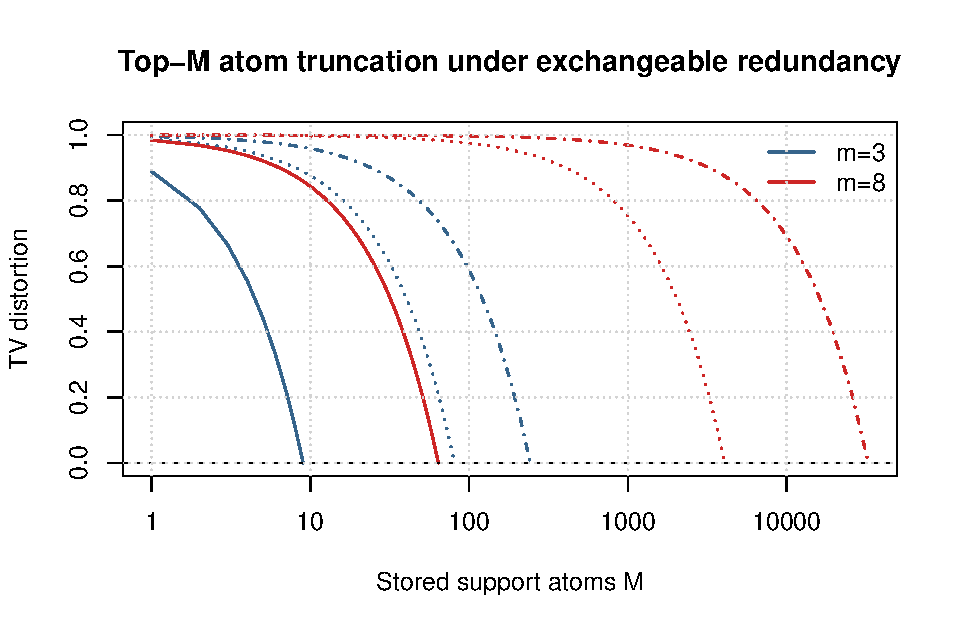
\includegraphics[width=.74\textwidth]{sim/output/figures/fig_topm_atom_separation.pdf}
\caption{TV distortion of top-\(M\) atom truncation under exchangeable group-representative redundancy. Region/kernel compression stores the exchangeable class as one region.}
\label{fig:maintopmsep}
\end{figure}

\subsection{Exact dictionary benchmark}
\label{subsec:currentexactcomparison}

Table~\ref{tab:maincompetitorbenchmark} is the full exact repeated benchmark for the two empirical questions. The reference target is exact unrestricted BMA, so TV, FKL, and RKL are measured without MCMC error. Each row selects the best FKL point for that method within its tuning grid and then averages over two correlations and five replications. The seven regimes cover one-representative redundancy, multi-representative redundancy, weak signals, noisy grouping, misspecified grouping, ordered interval structure, and graph communities. In the one-representative regime, each active redundant group has one signal coordinate. In the multi-representative regime, a group can contain several signal coordinates.

The result supports density-ratio compression as a checking framework. It does not show that one dictionary dominates every metric. Against methods outside the framework, the density-ratio-checked dictionary families give the best or near-best posterior-compression tradeoffs in most regimes. Dilution-prior BMA is strongest in the ordered-interval and weak-signal regimes, but it does so by changing the prior target.

Within the framework, pooled-pruned support kernels give consistently low FKL with \(q_0\) near the minimum fallback weight and moderate descriptor cost across all seven regimes. Posterior-cluster kernels are strong raw-distortion summaries. They can match or improve FKL in some regimes, but their storage includes learned medoids and bandwidths. Their larger \(q_0\) values also mean that the fallback component is doing more work. Top-\(M\) atoms and credible support sets can be TV-competitive in small exact settings, but they store atoms rather than regions. DPP-prior BMA is a useful redundancy-aware Bayesian comparison, but in these exact runs it is generally farther from unrestricted BMA than pooled-pruned support kernels.

\begin{table}[!tbp]
\centering
\scriptsize
\begin{tabular}{llcccc}
\toprule
Scenario & Method & TV & FKL & $q_0$ & Code \\
\midrule
graph community & Pooled-pruned & 0.014 (0.001) & 0.001 (0.000) & 0.001 (0.000) & 4.86 (0.17) \\
 & Cluster kernels & 0.025 (0.002) & 0.003 (0.000) & 0.207 (0.075) & 6.50 (0.35) \\
 & Top-M & 0.084 (0.017) & 0.040 (0.004) & 0.405 (0.086) & 29.75 (4.33) \\
 & Credible set & 0.041 (0.000) & 0.049 (0.000) & 0.164 (0.001) & 17.78 (0.27) \\
 & Dilution & 0.031 (0.003) & 0.006 (0.001) & -- & 43.50 (9.10) \\
 & DPP & 0.055 (0.005) & 0.021 (0.004) & -- & 37.10 (7.52) \\
 & Fixed hard & 0.048 (0.001) & 0.012 (0.001) & 0.652 (0.041) & 16.34 (0.70) \\
\addlinespace
misspecified grouping & Pooled-pruned & 0.011 (0.001) & 0.002 (0.000) & 0.001 (0.000) & 3.56 (0.16) \\
 & Cluster kernels & 0.013 (0.002) & 0.002 (0.000) & 0.025 (0.006) & 4.99 (0.10) \\
 & Top-M & 0.010 (0.004) & 0.019 (0.005) & 0.039 (0.014) & 9.88 (0.73) \\
 & Credible set & 0.040 (0.000) & 0.048 (0.000) & 0.156 (0.002) & 15.88 (0.14) \\
 & Dilution & 0.030 (0.006) & 0.006 (0.002) & -- & 8.80 (1.95) \\
 & DPP & 0.052 (0.011) & 0.022 (0.007) & -- & 7.20 (1.60) \\
 & Fixed hard & 0.025 (0.007) & 0.007 (0.003) & 0.801 (0.081) & 18.78 (1.38) \\
\addlinespace
multi representative & Pooled-pruned & 0.014 (0.002) & 0.002 (0.000) & 0.001 (0.000) & 4.65 (0.11) \\
 & Cluster kernels & 0.021 (0.001) & 0.002 (0.000) & 0.050 (0.029) & 5.53 (0.13) \\
 & Top-M & 0.014 (0.005) & 0.023 (0.005) & 0.052 (0.019) & 11.15 (0.87) \\
 & Credible set & 0.040 (0.000) & 0.048 (0.000) & 0.157 (0.001) & 16.44 (0.24) \\
 & Dilution & 0.038 (0.006) & 0.007 (0.002) & -- & 11.70 (2.75) \\
 & DPP & 0.069 (0.010) & 0.025 (0.006) & -- & 9.80 (2.14) \\
 & Fixed hard & 0.016 (0.003) & 0.010 (0.001) & 0.089 (0.036) & 6.53 (0.61) \\
\addlinespace
noisy grouping & Pooled-pruned & 0.013 (0.000) & 0.002 (0.000) & 0.001 (0.000) & 3.82 (0.29) \\
 & Cluster kernels & 0.016 (0.002) & 0.002 (0.000) & 0.035 (0.013) & 5.35 (0.16) \\
 & Top-M & 0.009 (0.003) & 0.017 (0.004) & 0.034 (0.013) & 9.76 (0.70) \\
 & Credible set & 0.039 (0.001) & 0.048 (0.000) & 0.155 (0.002) & 15.92 (0.30) \\
 & Dilution & 0.023 (0.005) & 0.005 (0.001) & -- & 8.50 (1.87) \\
 & DPP & 0.040 (0.007) & 0.017 (0.005) & -- & 6.70 (1.51) \\
 & Fixed hard & 0.025 (0.007) & 0.009 (0.003) & 0.729 (0.088) & 17.52 (1.52) \\
\addlinespace
one representative & Pooled-pruned & 0.017 (0.001) & 0.003 (0.000) & 0.001 (0.000) & 4.05 (0.17) \\
 & Cluster kernels & 0.019 (0.001) & 0.002 (0.000) & 0.026 (0.008) & 5.59 (0.11) \\
 & Top-M & 0.009 (0.003) & 0.018 (0.005) & 0.035 (0.013) & 9.54 (0.70) \\
 & Credible set & 0.039 (0.001) & 0.048 (0.000) & 0.154 (0.002) & 15.63 (0.12) \\
 & Dilution & 0.021 (0.004) & 0.004 (0.001) & -- & 8.50 (1.83) \\
 & DPP & 0.037 (0.006) & 0.015 (0.004) & -- & 7.10 (1.52) \\
 & Fixed hard & 0.046 (0.002) & 0.017 (0.001) & 0.506 (0.023) & 13.63 (0.41) \\
\addlinespace
ordered interval & Pooled-pruned & 0.016 (0.001) & 0.003 (0.000) & 0.001 (0.000) & 5.13 (0.03) \\
 & Cluster kernels & 0.030 (0.003) & 0.007 (0.000) & 0.284 (0.097) & 7.62 (0.27) \\
 & Top-M & 0.004 (0.001) & 0.009 (0.003) & 0.012 (0.006) & 7.83 (0.29) \\
 & Credible set & 0.039 (0.001) & 0.048 (0.000) & 0.152 (0.003) & 15.09 (0.26) \\
 & Dilution & 0.007 (0.003) & 0.000 (0.000) & -- & 5.10 (0.97) \\
 & DPP & 0.015 (0.006) & 0.002 (0.001) & -- & 5.10 (0.97) \\
 & Fixed hard & 0.065 (0.007) & 0.065 (0.006) & 0.006 (0.003) & 12.53 (0.15) \\
\addlinespace
weak signal & Pooled-pruned & 0.012 (0.001) & 0.003 (0.000) & 0.001 (0.000) & 2.76 (0.30) \\
 & Cluster kernels & 0.026 (0.003) & 0.004 (0.001) & 0.043 (0.011) & 4.12 (0.30) \\
 & Top-M & 0.047 (0.014) & 0.040 (0.003) & 0.212 (0.080) & 15.96 (4.62) \\
 & Credible set & 0.041 (0.000) & 0.052 (0.000) & 0.151 (0.002) & 12.81 (0.62) \\
 & Dilution & 0.011 (0.003) & 0.002 (0.001) & -- & 28.20 (5.55) \\
 & DPP & 0.019 (0.005) & 0.009 (0.003) & -- & 24.60 (4.42) \\
 & Fixed hard & 0.042 (0.002) & 0.019 (0.000) & 0.302 (0.043) & 9.86 (0.80) \\
\bottomrule
\end{tabular}

\caption{Exact dictionary benchmark. Parentheses give standard errors. Dilution and DPP rows change the prior target, so their TV and FKL values are target-shift diagnostics rather than compression errors.}
\label{tab:maincompetitorbenchmark}
\end{table}

\begin{table}[!htbp]
\centering
\scriptsize
\begin{tabular}{llccc}
\toprule
Scenario & Method & RMSE gap & Log-score gap & Selected \\
\midrule
graph community & Elastic net & -0.031 (0.011) & 0.007 (0.008) & 8.6 (0.5) \\
 & Group lasso & -0.025 (0.010) & -0.002 (0.009) & 4.0 (0.0) \\
 & Lasso & -0.030 (0.012) & 0.005 (0.009) & 8.3 (0.6) \\
\addlinespace
misspecified grouping & Elastic net & 0.033 (0.012) & -0.045 (0.011) & 7.2 (0.5) \\
 & Group lasso & 0.045 (0.014) & -0.065 (0.016) & 3.6 (0.2) \\
 & Lasso & 0.027 (0.010) & -0.041 (0.009) & 6.5 (0.6) \\
\addlinespace
multi representative & Elastic net & -0.027 (0.008) & -0.002 (0.012) & 8.7 (0.4) \\
 & Group lasso & 0.010 (0.015) & -0.041 (0.020) & 3.8 (0.1) \\
 & Lasso & -0.002 (0.019) & -0.027 (0.019) & 8.5 (0.8) \\
\addlinespace
noisy grouping & Elastic net & 0.042 (0.013) & -0.046 (0.010) & 8.6 (0.6) \\
 & Group lasso & 0.064 (0.013) & -0.072 (0.014) & 3.8 (0.1) \\
 & Lasso & 0.034 (0.012) & -0.035 (0.010) & 7.3 (0.6) \\
\addlinespace
one representative & Elastic net & 0.035 (0.013) & -0.038 (0.011) & 8.4 (0.5) \\
 & Group lasso & 0.073 (0.020) & -0.075 (0.017) & 3.9 (0.1) \\
 & Lasso & 0.023 (0.013) & -0.033 (0.014) & 8.1 (0.7) \\
\addlinespace
ordered interval & Elastic net & 0.005 (0.013) & -0.020 (0.013) & 6.6 (0.6) \\
 & Group lasso & 0.002 (0.010) & -0.015 (0.010) & 5.2 (0.6) \\
 & Lasso & 0.004 (0.012) & -0.017 (0.011) & 6.2 (0.7) \\
\addlinespace
weak signal & Elastic net & -0.063 (0.015) & 0.024 (0.008) & 6.3 (0.6) \\
 & Group lasso & 0.005 (0.013) & -0.027 (0.012) & 3.7 (0.2) \\
 & Lasso & -0.048 (0.015) & 0.017 (0.009) & 5.4 (0.6) \\
\bottomrule
\end{tabular}

\caption{Prediction-only baselines in the exact benchmark. Gaps are relative to reference BMA. These methods do not define compressed support posteriors, so TV and FKL are not applicable.}
\label{tab:exactpredictivebaselines}
\end{table}

\begin{figure}[!htbp]
\centering
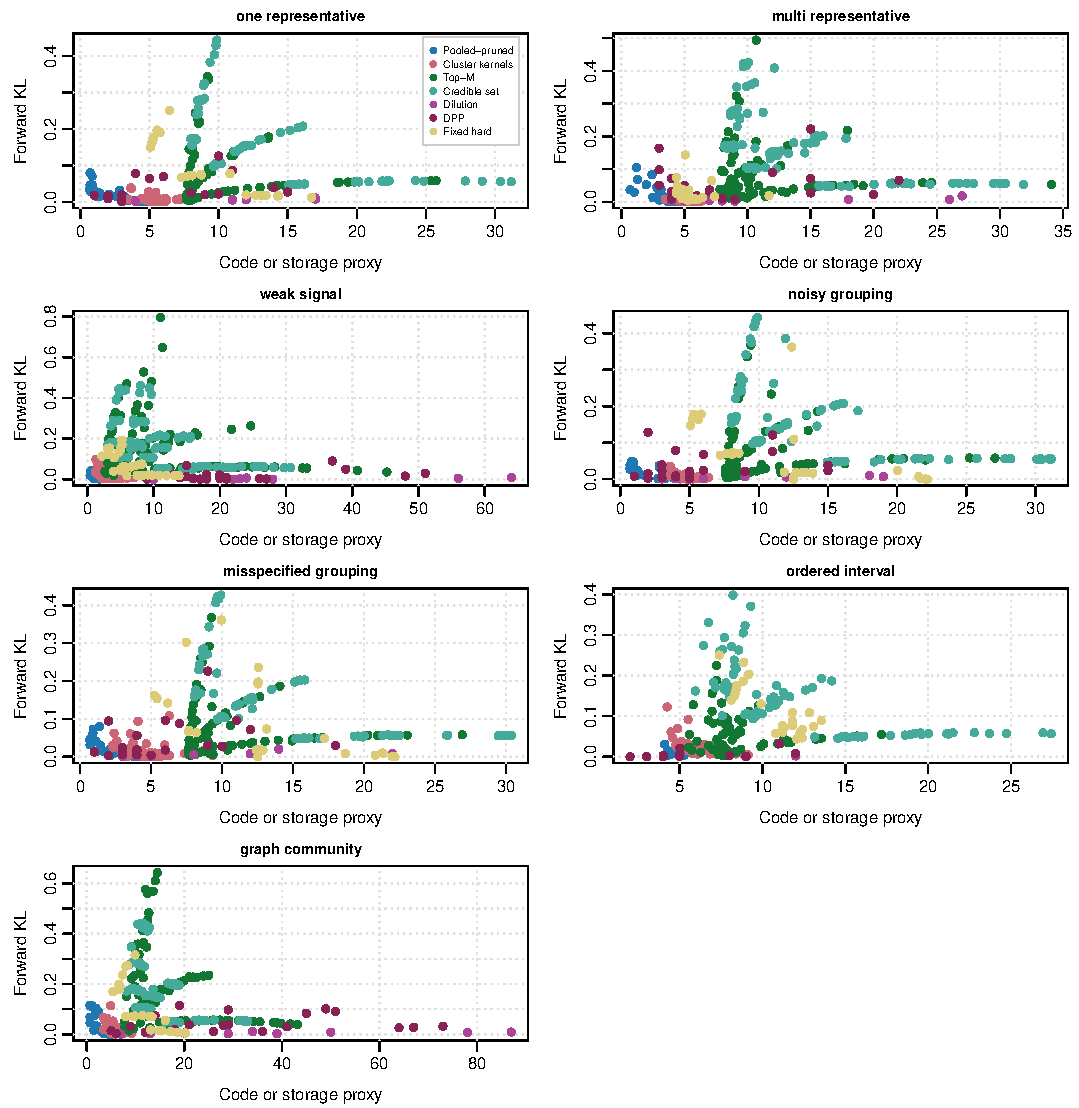
\includegraphics[width=.95\textwidth]{sim/output/figures/fig_support_kernel_competitor_frontier.pdf}
\caption{Exact fixed-target storage-distortion frontier.}
\label{fig:maincompetitorfrontier}
\end{figure}

\smallskip\noindent\textbf{Non-Gaussian check.} Table~\ref{tab:logisticcheck} repeats the compression step for a binary logistic support posterior. The reference posterior is computed by exact support enumeration with a Laplace approximation to the Gaussian-slab logistic marginal likelihood. The logistic experiment checks the support-posterior compression algebra beyond the Gaussian benchmark. It is not a full empirical study of GLM BMA. Its purpose is limited but important. Once a support posterior exists, support kernels, density ratios, TV, FKL, and \(q_0\) are computed in the same way as in the Gaussian experiments.

\begin{table}[!htbp]
\centering
\small
\begin{tabular}{lccccc}
\toprule
Method & TV & FKL & $q_0$ & Storage & Active \\
\midrule
Pooled-pruned & 0.054 (0.006) & 0.014 (0.002) & 0.001 (0.000) & 3.74 (0.06) & 9.3 (2.4) \\
Cluster kernels & 0.029 (0.007) & 0.005 (0.003) & 0.003 (0.001) & 4.83 (0.33) & 12.7 (1.9) \\
Top-M atoms & 0.209 (0.011) & 0.226 (0.004) & 0.215 (0.013) & 19.07 (0.70) & 33.0 (0.0) \\
Credible set & 0.050 (0.000) & 0.107 (0.000) & 0.047 (0.000) & 10.90 (0.27) & 102.0 (2.3) \\
Fixed regions & 0.157 (0.001) & 0.060 (0.002) & 0.620 (0.013) & 15.64 (0.25) & 4.3 (0.7) \\
\bottomrule
\end{tabular}

\caption{Small logistic support-posterior algebra check. This is not a full GLM BMA benchmark.}
\label{tab:logisticcheck}
\end{table}

\subsection{Large p=100 benchmark}
\label{subsec:largeendtoend}

The exact benchmark isolates the compression problem from posterior-sampling error. The next benchmark keeps the same comparison logic but moves to non-enumerable \(p=100\) support spaces. Each cell generates a synthetic redundant regression problem and runs six-chain MC3 to obtain an empirical unrestricted BMA reference posterior. It records reference-posterior diagnostics before compression is interpreted. It then compares pooled-pruned support kernels with top-\(M\) atoms, credible support sets, cluster kernels, dilution-prior BMA and DPP-prior BMA over the visited support set, and fixed hard-region lists. The full rerun contains \(12\) scenario-correlation cells with three replications each.

Table~\ref{tab:largeendtoenddiag} appears before the method summary because the reference posterior is the object being compressed. Compression metrics should not be read as high-confidence diagnostics when the reference sample itself is unstable. The final rerun uses \(18{,}000\) retained draws per cell. All \(36\) reference fits pass the core diagnostic gate, and one cell has a low-acceptance warning despite stable split-\(\widehat R\), ESS, and group-PIP diagnostics. This makes the large benchmark an end-to-end validation of the reported density-ratio posterior-compression layer, not only a saved-draw check.

\begin{table}[!htbp]
\centering
\small
\input{sim/output/tables/table_large_end_to_end_reference_diagnostics.tex}
\caption{Reference diagnostics for the large \(p=100\) benchmark.}
\label{tab:largeendtoenddiag}
\end{table}

The reference-posterior computation is the main additional cost before compression. In the full \(p=100\) rerun each reference fit used six MC3 chains, \(20{,}000\) iterations per chain, \(5{,}000\) burn-in iterations, and thinning by \(5\), giving \(18{,}000\) retained cold-chain draws per cell. The mean reference runtime was \(21.1\) seconds per cell, with range \(11.7\) to \(33.7\) seconds on the benchmark workstation. These timings are not meant as a universal speed claim. They quantify the reference-posterior overhead for the reported benchmark and explain why the diagnostic gate is shown before the compression table.

Conditional on these reference samples, Table~\ref{tab:largeendtoendmethods} supports the intended rate-distortion claim. Pooled-pruned support kernels have lower FKL and lower expected descriptor cost than top-\(M\) atoms, dilution-prior BMA, DPP-prior BMA, credible support sets, and fixed hard regions. The Storage column is \(C_{\mathrm{exp}}\). The List column reports active kernels or stored atoms. The large List value for pooled-pruned is a warning that the refitted mixture still uses many small-weight descriptors, even though its expected code is low.

Cluster kernels give the lowest raw TV and FKL in the large run, but they leave much larger fallback weight and require reporting learned medoids, bandwidths, and cluster counts. Thus the large benchmark does not show uniform domination. It supports the broader framework view. Different kernel dictionaries can be checked on the same density-ratio scale. The user can choose the low expected-code pooled-pruned summary or the raw-distortion cluster summary according to the reporting goal.

\begin{table}[!htbp]
\centering
\scriptsize
\begin{tabular}{lcccccc}
\toprule
Method & TV & FKL & $q_0$ & Storage & List & RMSE gap \\
\midrule
Pooled-pruned & 0.076 (0.002) & 0.017 (0.001) & 0.334 (0.030) & 11.32 (0.36) & 137.1 (19.5) & 0.001 (0.001) \\
Cluster kernels & 0.049 (0.002) & 0.007 (0.001) & 0.723 (0.018) & 16.42 (0.20) & 13.9 (0.5) & 0.001 (0.000) \\
Top-M atoms & 0.220 (0.033) & 0.486 (0.049) & 0.050 (0.008) & 69.06 (6.39) & 96.0 (0.0) & 0.005 (0.002) \\
Credible set & 0.103 (0.001) & 0.427 (0.001) & 0.006 (0.000) & 29.34 (1.30) & 639.8 (244.4) & 0.003 (0.001) \\
Dilution BMA & 0.170 (0.017) & 0.407 (0.065) & -- & 318.47 (84.24) & 318.5 (84.2) & 0.004 (0.001) \\
DPP BMA & 0.185 (0.018) & 0.439 (0.069) & -- & 305.11 (82.07) & 305.1 (82.1) & 0.005 (0.001) \\
Fixed regions & 0.189 (0.027) & 0.188 (0.027) & 0.343 (0.069) & 94.33 (15.57) & 38.1 (2.7) & 0.003 (0.001) \\
\bottomrule
\end{tabular}

\caption{Large \(p=100\) benchmark. Storage is expected descriptor cost, and List is active kernels or stored atoms. Dilution and DPP rows change the prior target, so their TV and FKL values are target-shift diagnostics.}
\label{tab:largeendtoendmethods}
\end{table}

\noindent Because low FKL can be obtained by leaving weight on the unrestricted fallback component, Table~\ref{tab:q0screenedfrontier} screens the same tuning grid by \(q_0\). This is not a separate constrained optimization run. It is a direct check of whether a dictionary family still works when large fallback solutions are excluded. Under the strict \(q_0\le0.05\) screen, pooled-pruned support kernels remain the strongest FKL row among the reported dictionary families. As the screen is relaxed, FKL improves and the active list grows. This makes the fallback-storage-distortion tradeoff part of the main evidence rather than a hidden tuning artifact.

\begin{table}[!htbp]
\centering
\small
\begin{tabular}{llcccc}
\toprule
$q_0$ screen & Method & cells & FKL & Storage & active/atoms \\
\midrule
$q_0\le0.05$ & Pooled-pruned & 36 & 0.056 (0.003) & 6.60 (0.06) & 60.5 \\
 & Cluster kernels & 31 & 0.172 (0.007) & 8.47 (0.25) & 14.3 \\
 & Top-M atoms & 36 & 0.687 (0.073) & 47.57 (1.73) & 92.1 \\
 & Fixed regions & 26 & 0.866 (0.103) & 25.77 (0.66) & 43.3 \\
\addlinespace
$q_0\le0.10$ & Pooled-pruned & 36 & 0.056 (0.003) & 6.63 (0.07) & 66.0 \\
 & Cluster kernels & 35 & 0.174 (0.008) & 8.78 (0.23) & 15.0 \\
 & Top-M atoms & 36 & 0.550 (0.062) & 62.21 (3.16) & 92.1 \\
 & Fixed regions & 36 & 0.613 (0.106) & 27.50 (0.99) & 35.5 \\
\addlinespace
$q_0\le0.25$ & Pooled-pruned & 36 & 0.049 (0.004) & 7.63 (0.27) & 87.6 \\
 & Cluster kernels & 36 & 0.140 (0.012) & 10.00 (0.22) & 17.6 \\
 & Top-M atoms & 36 & 0.486 (0.031) & 69.06 (4.14) & 92.1 \\
 & Fixed regions & 36 & 0.332 (0.059) & 52.32 (2.73) & 36.2 \\
\addlinespace
$q_0\le0.50$ & Pooled-pruned & 36 & 0.027 (0.004) & 10.36 (0.28) & 132.8 \\
 & Cluster kernels & 36 & 0.070 (0.009) & 12.24 (0.25) & 16.5 \\
 & Top-M atoms & 36 & 0.486 (0.031) & 69.06 (4.14) & 92.1 \\
 & Fixed regions & 36 & 0.259 (0.049) & 59.96 (3.70) & 36.0 \\
\bottomrule
\end{tabular}

\caption{\(q_0\)-screened large \(p=100\) frontier. Rows select the best available tuning-grid fit satisfying the displayed fallback screen. They are not solutions of a separate constrained optimization problem.}
\label{tab:q0screenedfrontier}
\end{table}

\begin{table}[!htbp]
\centering
\small
\begin{tabular}{lccc}
\toprule
Method & RMSE gap & Log-score gap & Selected \\
\midrule
Elastic net & 0.008 (0.018) & -0.087 (0.033) & 25.5 (2.2) \\
Group lasso & 0.107 (0.022) & -0.244 (0.048) & 11.7 (1.3) \\
Lasso & 0.001 (0.015) & -0.070 (0.028) & 19.9 (2.5) \\
\bottomrule
\end{tabular}

\caption{Prediction-only baselines in the large \(p=100\) benchmark. These methods do not define compressed support posteriors, so TV and FKL are not applicable.}
\label{tab:largepredictivebaselines}
\end{table}

\subsection{Dictionary diagnostics}
\label{subsec:ablationdiagnostics}

The remaining diagnostics ask how the candidate generator behaves. The full candidate-source table is in Appendix Table~\ref{tab:adaptiveablationdetail}, because it is a medium-mode diagnostic rather than main evidence. Its message is simple. Cluster-only and residual-only sources can give the smallest raw FKL or TV in the easy high-redundancy setting. Pooled-union and \(99\%\) \(q\)-pruned rows diagnose whether the finite candidate pool is rich, but their active-list sizes show that they are not automatically short descriptor lists. The implementation also checks the embedded pruned solution inside the pooled list, so the pooled diagnostic is not allowed to be worse than its pruned subset under the same objective.

Table~\ref{tab:mainadaptiveconv} reports one representative sequential trace. The penalized objective drops as columns are added. Raw distortion and expected code can move in different directions, which is why the main tables report both distortion and storage diagnostics.

\begin{table}[!htbp]
\centering
\scriptsize
\begin{tabular}{rrrrrrrrr}
\toprule
Iter. & Obj. & FKL & TV & $q_0$ & Code & Active & Best score & KKT \\
\midrule
1 & 0.200 & 0.000 & 0.000 & 1.000 & 10.000 & 1 & 0.186 & 0.000 \\
2 & 0.121 & 0.042 & 0.122 & 0.352 & 3.965 & 2 & 0.409 & 0.017 \\
4 & 0.102 & 0.052 & 0.110 & 0.123 & 2.503 & 4 & 0.267 & 0.004 \\
6 & 0.095 & 0.049 & 0.101 & 0.079 & 2.330 & 6 & 0.118 & 0.004 \\
8 & 0.087 & 0.041 & 0.095 & 0.039 & 2.336 & 8 & 0.051 & 0.055 \\
10 & 0.075 & 0.023 & 0.074 & 0.001 & 2.689 & 10 & -0.002 & 0.018 \\
\bottomrule
\end{tabular}

\caption{Sequential column-generation trace for the fixed-target compression objective.}
\label{tab:mainadaptiveconv}
\end{table}

\subsection{Applied checks}
\label{subsec:largersaveddraw}

\smallskip\noindent\textbf{Saved-draw check.} Table~\ref{tab:mainadaptivep100} keeps the older saved-draw \(p=100\) check as a secondary diagnostic. Unlike the end-to-end run in Section~\ref{subsec:largeendtoend}, this table evaluates compression on stored unrestricted BMA posterior draws rather than rerunning the reference sampler and predictive splits. It is therefore useful for checking structured support kernels in a larger support space, but it is not the main large-\(p\) evidence. The pooled-pruned dictionaries reduce TV and forward KL relative to fixed hard-region lists across the displayed scenarios, while nonzero \(q_0\) values indicate partial rather than complete compression.

\begin{table}[!htbp]
\centering
\scriptsize
\begin{tabular}{llrrrrr}
\toprule
Scenario & Method & TV & FKL & $q_0$ & Code & Kernels \\
\midrule
multi\_representative & Adaptive kernel & 0.111 & 0.043 & 0.533 & 13.811 & 7.0 \\
noisy\_grouping & Adaptive kernel & 0.113 & 0.041 & 0.613 & 14.623 & 7.0 \\
one\_representative & Adaptive kernel & 0.123 & 0.049 & 0.484 & 13.337 & 7.0 \\
weak\_signal & Adaptive kernel & 0.164 & 0.087 & 0.416 & 10.044 & 5.0 \\
multi\_representative & Fixed hard & 0.388 & 0.698 & 0.075 & 37.284 & 65.0 \\
noisy\_grouping & Fixed hard & 0.539 & 1.002 & 0.133 & 46.454 & 65.0 \\
one\_representative & Fixed hard & 0.336 & 0.624 & 0.055 & 33.307 & 64.0 \\
weak\_signal & Fixed hard & 0.350 & 0.664 & 0.056 & 30.391 & 65.0 \\
\bottomrule
\end{tabular}

\caption{Saved-draw \(p=100\) fixed-target density-ratio posterior compression.}
\label{tab:mainadaptivep100}
\end{table}

\smallskip\noindent\textbf{Semi-synthetic Tecator.}

The semi-synthetic spectroscopy experiment uses the real Tecator predictor matrix with a known simulated banded signal. This keeps the difficult part of the design, since adjacent wavelength channels are highly correlated. It also gives a known active region for checking interpretability. Table~\ref{tab:mainsemisynth} and Figure~\ref{fig:mainsemisynth} show that structured pooled-pruned support kernels improve TV and forward KL over fixed hard-region lists and top-\(M\) atoms at low expected descriptor cost, with negligible predictive degradation. The learned high-weight kernels also overlap the simulated active band. This is the strongest controlled practical evidence in the paper. The response is simulated and the reduced posterior is easier to validate, so the result should be read as controlled validation rather than as a production benchmark.

\begin{table}[!htbp]
\centering
\begin{tabular}{lrrrrrr}
\toprule
Method & TV & FKL & $q_0$ & Reporting cost & RMSE gap & Kernels \\
\midrule
Adaptive kernel & 0.058 & 0.017 & 0.001 & 2.348 & 0.0001 & 7.3 \\
Fixed hard & 0.071 & 0.027 & 0.012 & 4.800 & 0.0001 & 17.0 \\
Top-$M$ atoms & 0.142 & 0.203 & 0.129 & 10.490 & 0.0004 & 33.0 \\
\bottomrule
\end{tabular}

\caption{Semi-synthetic real-\(X\) Tecator fixed-target compression with simulated response.}
\label{tab:mainsemisynth}
\end{table}

\begin{figure}[H]
\centering
\begin{tabular}{@{}cc@{}}
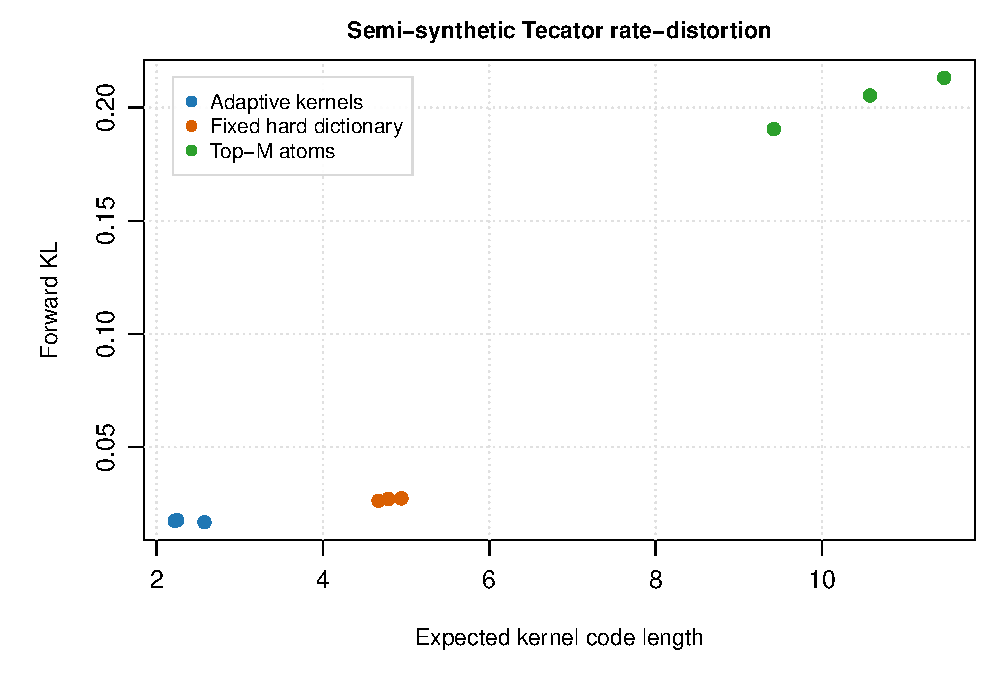
\includegraphics[width=.47\textwidth]{sim/output/figures/fig_adaptive_kernel_semisynthetic_realx.pdf} &
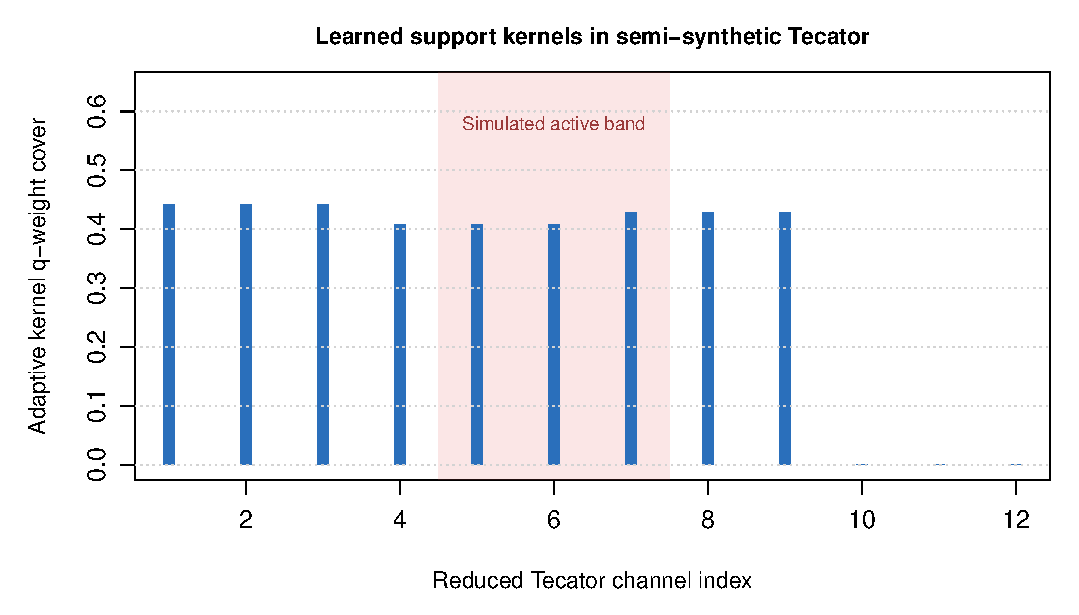
\includegraphics[width=.47\textwidth]{sim/output/figures/fig_semisynthetic_tecator_kernels.pdf}
\end{tabular}
\caption{Semi-synthetic Tecator diagnostics. The shaded band marks the simulated active channels. Blue bars show \(q\)-weighted coverage by high-weight non-fallback kernels.}
\label{fig:mainsemisynth}
\end{figure}

\smallskip\noindent\textbf{Reduced exact real-response spectroscopy.}
\label{subsec:realresponsereduced}

The final experiment uses real spectroscopy predictors and real responses. We use Tecator meat spectroscopy with fat response and Gasoline near-infrared spectra with octane response \citep{thodberg1993,liland2026pls}. Both data sets have ordered, highly redundant spectral channels, so they match the support-region story of the paper. To avoid centering the evidence on a weak full-resolution MCMC reference posterior, we construct a reduced ordered-region design by averaging contiguous spectral blocks using only \(X\). We then enumerate the exact BMA posterior on those regions. This is not a claim about full-resolution spectroscopy. It is a real-response, real-design test of density-ratio posterior compression under a reference posterior that is exact by construction.

Table~\ref{tab:realresponseexact} reports Tecator fat and Gasoline octane results. The same posterior compression competitors are used as in the exact synthetic benchmark. Lasso, elastic net, and group lasso rows are kept as prediction checks. The real-response dilution row uses the powered determinant correction, and the DPP row uses the determinant prior with unit power. This experiment tests whether the learned region summaries remain useful when both \(X\) and \(y\) come from real data. It also makes the earlier diagnostic lesson operational. Real-data rows should not be central evidence unless the reference posterior is trustworthy. Here the trust comes from exact enumeration after a deterministic spectral reduction, not from an uncertain sampler.

The reduced real-response results are modest in scope, but they are not a stress-test failure. Pooled-pruned support kernels have lower FKL than Top-\(M\) atoms, credible support sets, dilution-prior BMA, DPP-prior BMA, and fixed hard regions on both data sets. Posterior-cluster kernels are again a strong raw-distortion competitor. On Tecator they give lower FKL, but with a much larger fallback weight and a learned-medoid reporting cost. Fixed hard regions can have competitive TV on Gasoline, but most of the mixture remains in the fallback component. These patterns match the synthetic benchmarks. Structured pooled-pruned regions are low expected-code checked summaries, while cluster kernels are useful when raw distortion is the main target.

\begin{table}[H]
\centering
\scriptsize
\begin{tabular}{llccccc}
\toprule
Dataset & Method & TV & FKL & $q_0$ & $C_{\mathrm{exp}}$ & RMSE gap \\
\midrule
Gasoline & Pooled-pruned & 0.067 (0.001) & 0.016 (0.000) & 0.001 (0.000) & 5.96 (0.04) & 0.000 (0.000) \\
 & Cluster kernels & 0.076 (0.003) & 0.019 (0.002) & 0.490 (0.058) & 8.10 (0.19) & 0.001 (0.001) \\
 & Top-M atoms & 0.231 (0.012) & 0.216 (0.003) & 0.271 (0.018) & 25.46 (0.86) & 0.003 (0.001) \\
 & Credible set & 0.090 (0.000) & 0.147 (0.000) & 0.098 (0.000) & 17.74 (0.11) & 0.001 (0.001) \\
 & Dilution BMA & 0.642 (0.010) & 1.899 (0.070) & -- & 72.00 (6.94) & 0.004 (0.004) \\
 & DPP BMA & 0.816 (0.015) & 5.571 (0.239) & -- & 31.40 (1.29) & 0.017 (0.007) \\
 & Fixed regions & 0.056 (0.011) & 0.026 (0.005) & 0.942 (0.012) & 41.01 (0.41) & -0.000 (0.000) \\
\addlinespace
Tecator & Pooled-pruned & 0.076 (0.002) & 0.022 (0.002) & 0.001 (0.000) & 6.45 (0.09) & -0.001 (0.001) \\
 & Cluster kernels & 0.053 (0.002) & 0.009 (0.001) & 0.570 (0.117) & 9.19 (0.19) & -0.003 (0.002) \\
 & Top-M atoms & 0.260 (0.009) & 0.219 (0.001) & 0.322 (0.018) & 28.24 (0.95) & -0.015 (0.004) \\
 & Credible set & 0.091 (0.000) & 0.146 (0.000) & 0.100 (0.001) & 18.63 (0.25) & -0.007 (0.002) \\
 & Dilution BMA & 0.904 (0.007) & 8.225 (0.308) & -- & 10.00 (0.45) & 0.052 (0.022) \\
 & DPP BMA & 0.984 (0.002) & 18.969 (0.477) & -- & 2.60 (0.24) & 0.058 (0.025) \\
 & Fixed regions & 0.157 (0.015) & 0.073 (0.007) & 0.816 (0.021) & 36.82 (0.70) & -0.006 (0.004) \\
\bottomrule
\end{tabular}

\caption{Reduced exact real-response spectroscopy benchmark. Dilution and DPP rows change the prior target, so their TV and FKL values are target-shift diagnostics. Prediction-only sparse rows do not define compressed support posteriors.}
\label{tab:realresponseexact}
\end{table}

Table~\ref{tab:keypairedcomparisons} summarizes paired comparisons for the main current outputs. The mean gap is comparison minus pooled-pruned, so positive FKL means pooled-pruned has lower forward KL, while positive storage means pooled-pruned has lower expected descriptor cost. The tests are not used as a binary decision rule, but they show that the main qualitative comparisons are not driven by one replication.

\begin{table}[H]
\centering
\footnotesize
\begin{tabular}{llcrr}
\toprule
Evidence & Comparison & metric & mean gap & Wilcoxon $p$ \\
\midrule
Exact & Top-M atoms & FKL & 0.021 & <0.001 \\
Exact & Posterior clustering & FKL & 0.001 & <0.001 \\
Exact & Posterior clustering & storage & 1.553 & <0.001 \\
Exact & Dilution-prior BMA & FKL & 0.002 & 0.002 \\
Large end-to-end & Top-M atoms & FKL & 0.469 & <0.001 \\
Large end-to-end & Posterior clustering & FKL & -0.011 & <0.001 \\
Large end-to-end & Posterior clustering & storage & 5.117 & <0.001 \\
Large end-to-end & Dilution-prior BMA & FKL & 0.390 & <0.001 \\
Reduced real-response & Top-M atoms & FKL & 0.198 & 0.006 \\
Reduced real-response & Posterior clustering & FKL & -0.006 & 0.103 \\
Reduced real-response & Posterior clustering & storage & 2.380 & 0.006 \\
\bottomrule
\end{tabular}

\caption{Paired comparison checks for key current outputs.}
\label{tab:keypairedcomparisons}
\end{table}

\smallskip\noindent\textbf{Reproducibility.} The companion GitHub repository contains the active R implementation, figure and table generators, fixed seeds, tuning grids, and benchmark scripts. Its README gives one-command paths for the exact benchmark, the large \(p=100\) end-to-end benchmark, the logistic check, the \(q_0\)-screened frontier, the reduced real-response spectroscopy benchmark, and PDF compilation. The large benchmark also stores reference-posterior diagnostics before compression is interpreted. The generated CSV files used by the manuscript tables and figures are regenerated from these scripts.

\section{Discussion}
\label{sec:discussion}

The paper contributes density-ratio posterior compression for a fixed unrestricted support posterior. The object being compressed is the posterior distribution over \(\Gamma_p\), not a particular Gaussian slab or linear likelihood. The Gaussian linear model is the worked benchmark because it lets us enumerate, sample, and diagnose the reference posterior. The exact density-ratio identities make TV, forward KL, reverse KL, predictive contraction, and \(q_0\) computable diagnostics rather than informal summaries. A dictionary can come from response-independent hard regions, structured adaptive kernels, posterior clusters, residual covers, pooled-pruned hybrids, or top posterior atoms. The same density-ratio calculation checks each approximation on held-out posterior draws.

The distinction between a Bayesian hierarchy and a posterior-adaptive summary is essential. Fixed response-independent hard families can be interpreted as a Bayesian hierarchy. Posterior-adaptive kernels learned from posterior samples are instead a compression approximation to an already fitted reference posterior. Sample splitting is what makes the latter honest.

The top-\(M\) comparison clarifies why support-region compression is not just posterior atom truncation with a new name. Under group-representative redundancy, top-\(M\) must store many individual supports, while a single region can preserve uncertainty among substitute supports inside the region. In small exact examples top-\(M\) can be TV-competitive, but it pays atom-list cost and does not provide the same low-resolution representation.

The theoretical results have two roles. The validation results say what is true once a reference posterior, a candidate pool, mass estimates, and a validation split are available. The assumption table turns these conditions into diagnostic checks. The structural results show concrete cases where the candidate pool can be rich enough. Separated Hamming-ball posterior clusters, group-representative regions, and ordered interval bands all give low-distortion support-kernel coverage under transparent conditions. Together with the atom-truncation lower bound, this explains why regions are the right object under group-representative redundancy. The theory does not solve posterior computation by itself, and it does not prove that every generated candidate pool contains the best low descriptor-cost representation. The contribution is an exact compression object, practical diagnostic gates, concrete redundancy regimes, and a way to reject inadequate summaries.

The empirical evidence follows the same logic. It includes exact enumerable checks, a full exact benchmark, a \(p=100\) end-to-end benchmark with \(36\) passing reference fits, \(q_0\)-screened frontiers, saved-draw diagnostics, ablations, semi-synthetic real-\(X\) validation, and reduced real-response spectroscopy checks with exact reference posteriors. The experiments answer two questions. First, density-ratio compression gives favorable posterior-compression tradeoffs against outside Bayesian baselines such as dilution-prior BMA and DPP-prior BMA in most reported regimes, while keeping the unrestricted posterior target fixed. Second, the best dictionary family depends on the reporting goal.

Posterior-cluster kernels are strong raw-distortion summaries and often have lower TV and FKL, but they use learned medoids and can leave a larger fallback weight. Pooled-pruned structured dictionaries are low expected-code, interpretable support-region summaries against Top-\(M\), credible-set, DPP-prior, and fixed-region comparisons. This is an expected-code claim, not a claim that the total active descriptor list is always smallest. The accompanying active-list and stored-atom columns expose code sensitivity. Dilution-prior BMA is competitive in some exact regimes, but it changes the prior target rather than compressing the fixed unrestricted posterior. The reduced real-response checks show practical use under exact references, while larger full-resolution real-response applications would be needed for broader applied claims. Broader computational claims would also require more large-\(p\) cells and independent stability checks, possibly through parallel tempering, SMC, annealed importance sampling, or another externally validated approximation.

This is a real limitation. The method is a compression and reporting layer for an unrestricted Bayesian analysis. It is useful after a reliable reference posterior, or a reliable approximation to it, has been obtained. It is not automatically faster than unrestricted BMA, and it should not be marketed as a scalable replacement for reference-posterior computation. A scalable replacement would require a separately validated support-MCMC, SMC, variational, or annealed reference-posterior engine with its own mixing, accuracy, and runtime evidence.

The same distinction applies to model classes. The theory only needs a support-indexed posterior and predictive kernel. Logistic, count, survival, grouped, and other regression BMA analyses can therefore be compressed by the same density-ratio calculation once their reference support posterior is available. Those extensions would need their own reference-posterior diagnostics and empirical benchmarks. The present paper establishes density-ratio posterior compression and tests it in the Gaussian linear instance where the support posterior can be checked most directly.

The comparison set should be read in the same way. The paper includes the most direct support-space comparisons from Section~\ref{subsec:benchmarktarget}. These are Top-\(M\) support truncation from ordinary BMA, posterior clustering or block-based summaries under collinearity, and dilution or powered-correlation priors. Our structural redundancy theory covers exact permutation redundancy and near-uniform support posterior mass. Primitive design-level perturbation bounds for near-duplicate predictors are left for future work. The benchmark is still not a final comparison against every adjacent ML workflow. A later broader study should compare against production projection predictive workflows, structured variational support approximations, and SMC or annealed reference posterior engines under the same TV/FKL/RKL, prediction, interpretability, runtime, and failure-diagnostic metrics.

Future work should improve reference posterior samplers, add richer overlapping and scientific module kernels, quantify region stability across sample splits, and develop larger-scale variational or SMC reference approximations. These are extensions of density-ratio posterior compression, not replacements for the central diagnostic principle. A low-resolution posterior representation should be learned and checked relative to a fixed unrestricted Bayesian analysis, and it should be rejected when the reference posterior, candidate pool, or held-out distortion diagnostics fail.

\section*{Acknowledgments}

Xuewen Lu gratefully acknowledges support from a Discovery Grant (RGPIN-2024-03951) from the Natural Sciences and Engineering Research Council (NSERC) of Canada.

\ifBMAincludeSupplement
\appendix

\section{Supporting Theory}
\label{app:supportingtheory}

This appendix collects supporting statements that are used by the main results but are not part of the main narrative.

\begin{proposition}[Hard-region ratio]
\label{prop:mixtureidentity}
For any region list in Definition~\ref{def:familydictionary} and any \(q\in\Delta_M\),
\[
\bar\pi_q(\gamma\mid\D)=\pi_0(\gamma\mid\D)h_q(\gamma), \qquad \E_{\pi_0}\{h_q(\Gamma)\}=1.
\]
Consequently,
\begin{align}
\KL\!\left(\bar\pi_q\,\|\,\pi_0\right)&=\E_{\pi_0}\!\left[h_q(\Gamma)\log h_q(\Gamma)\right], \label{eq:mixtureRKL}\\
\TV\!\left(\bar\pi_q,\pi_0\right)&=\frac12\E_{\pi_0}\!\left[|h_q(\Gamma)-1|\right]. \label{eq:mixtureTV}
\end{align}
If $h_q(\gamma)>0$ for $\pi_0$-almost every $\gamma$, then
\begin{equation}
\KL\!\left(\pi_0\,\|\,\bar\pi_q\right) = \E_{\pi_0}\!\left[-\log h_q(\Gamma)\right]. \label{eq:mixtureFKL}
\end{equation}
For every fixed prediction point $\tilde x$,
\[
\TV\!\left(p_{\bar\pi_q}(\cdot\mid\tilde x,\D),p_{\pi_0}(\cdot\mid\tilde x,\D)\right) \le \TV\!\left(\bar\pi_q,\pi_0\right).
\]
\end{proposition}

\begin{corollary}[Fallback weight]
\label{cor:safetyresidue}
For any \(q\in\Delta_M\), the fallback region contributes \(q_0\pi_0(\cdot\mid\D)\) to \(\bar\pi_q\). If a low expected-code solution has small \(q_0\) and small TV or KL distortion, then the region list compresses the unrestricted support posterior under that distortion. If every low expected-code solution has large \(q_0\) or large distortion, then the region list has failed to give a useful low-resolution representation of the posterior. Thus \(q_0\) is a fallback diagnostic, not a posterior probability that a scientific group is active.
\end{corollary}

\begin{proposition}[Reference error transfer]
\label{prop:referenceerror}
Let \(\pi_\star\) be the ideal unrestricted BMA posterior and let \(\pi_0\) be the reference posterior used to build and check \(\bar\pi_q^{\,W}\). If \(\TV(\pi_0,\pi_\star)\le\eta\), then
\[
\TV(\bar\pi_q^{\,W},\pi_\star) \le \TV(\bar\pi_q^{\,W},\pi_0)+\eta .
\]
Consequently, for every \(|\varphi|\le B\),
\[
\left| \E_{\bar\pi_q^{\,W}}\varphi-\E_{\pi_\star}\varphi \right| \le 2B\{\TV(\bar\pi_q^{\,W},\pi_0)+\eta\}.
\]
The same bound holds after applying any common posterior-predictive Markov kernel. Thus a small density-ratio diagnostic relative to \(\pi_0\) transfers to the target posterior only to the extent that the reference posterior itself has been validated.
\end{proposition}

\begin{proposition}[MCMC check]
\label{prop:mixingcertification}
Condition on two events. The construction split is fixed, and the alpha-estimation event in Theorem~\ref{thm:empiricalcertification} holds. Let the validation output \(\Gamma_{1:N}\) be a stationary beta-mixing sequence from \(\pi_0(\cdot\mid\D)\) with coefficients \(\beta_{\mathrm{mix}}(k)\). Suppose \(N=2\mu b\). Split the output into \(2\mu\) consecutive blocks of length \(b\), keep the odd blocks, and define the blocked validation objective by replacing \(N^{-1}\sum_i\ell\{\widehat h_q(\Gamma_i)\}\) with the average of the \(\mu\) odd-block means. Let \(\widehat q_b\) minimize this blocked objective over the same feasible set \(\mathcal Q\) as in Theorem~\ref{thm:empiricalcertification}. Under the same boundedness and Lipschitz assumptions, with probability at least \(1-\delta-(\mu-1)\beta_{\mathrm{mix}}(b)\),
\[
\mathcal L_{\beta,\tau}^a(\widehat q_b) \le \inf_{q\in\mathcal Q}\mathcal L_{\beta,\tau}^a(q) + 4La^{-1}\sqrt{\frac{2\log\{2(M+1)\}}{\mu}} + 2B_\ell\sqrt{\frac{\log(2/\delta)}{2\mu}} + 2L r_\alpha .
\]
\end{proposition}

\begin{corollary}[Finite-pool check]
\label{cor:endtoendcertification}
Condition on the construction split and on a finite candidate pool \(\mathcal W=\{w_0,\dots,w_J\}\) containing the fallback kernel \(w_0\equiv1\). Let all retained masses be lower bounded by the floor \(a\), and let validation and alpha-estimation samples be independent of the construction split. Suppose the active-set solver returns \(\widehat q\in\Delta_{\epsilon_0}\) with empirical finite-pool optimization gap
\[
\widehat{\mathcal L}_{\beta,\tau}(\widehat q) \le \inf_{q\in\Delta_{\epsilon_0}^{J}} \widehat{\mathcal L}_{\beta,\tau}(q) + \varepsilon_{\mathrm{opt}},
\]
where \(\Delta_{\epsilon_0}^{J}\) is the simplex over the finite pool with fallback weight \(q_0\ge\epsilon_0\). Under the assumptions of Theorem~\ref{thm:empiricalcertification}, and on the reciprocal mass-estimation event with radius \(r_\alpha\), with probability at least \(1-\delta\) over the validation sample,
\[
\mathcal L_{\beta,\tau}^a(\widehat q) \le \inf_{q\in\Delta_{\epsilon_0}^{J}} \mathcal L_{\beta,\tau}^a(q) + \varepsilon_{\mathrm{opt}} + 4La^{-1}\sqrt{\frac{2\log\{2(J+1)\}}{N}} + 2B_\ell\sqrt{\frac{\log(2/\delta)}{2N}} + 2L r_\alpha .
\]
If the finite pool is itself a generated subset of a larger ideal comparison class \(\mathfrak W\), the corollary leaves a candidate-class approximation term between the best generated-pool mixture and the best mixture in that larger class.
\end{corollary}

\begin{theorem}[Cluster cover]
\label{thm:clustercoverage}
Let \(d\) be Hamming distance or group-Hamming distance on \(\Gamma_p\). Suppose there are centers \(c_1,\dots,c_K\), radius \(R\), and posterior balls \(B_r=\{\gamma:d(\gamma,c_r)\le R\}\) such that
\[
\pi_0\left(\bigcup_{r=1}^K B_r\mid\D\right)\ge1-\varepsilon, \qquad \pi_0(B_r\mid\D)=p_r>0,
\]
and \(d(c_r,c_s)>6R\) for \(r\ne s\). Draw \(N_c\) construction supports iid from \(\pi_0(\cdot\mid\D)\). Suppose the cluster-kernel generator returns one observed center \(\widehat c_r\in B_r\) whenever the construction sample hits \(B_r\), and includes the hard ball kernel
\[
\widehat w_r(\gamma)=\ind\{d(\gamma,\widehat c_r)\le2R\}.
\]
Then with probability at least \(1-\sum_{r=1}^K\exp(-N_c p_r)\), the generated pool contains disjoint kernels whose union has retained mass at least \(1-\varepsilon\). On this event, for every \(\zeta\in[\epsilon_0,1)\) there is a feasible mixture over those kernels and the fallback kernel such that
\[
\TV(\bar\pi_q^{\,W},\pi_0)\le(1-\zeta)\varepsilon, \qquad \KL(\pi_0\,\|\,\bar\pi_q^{\,W})\le\varepsilon\log(1/\zeta).
\]
\end{theorem}

\begin{lemma}[Mass estimation]
\label{lem:alphaestimation}
Suppose
\[
\widehat\alpha_m = N_\alpha^{-1}\sum_{i=1}^{N_\alpha}w_m(\Gamma_i^\alpha)
\]
is computed from an independent iid alpha-estimation sample from $\pi_0(\cdot\mid\D)$ for kernels $0\le w_m\le1$. With probability at least $1-\delta$,
\[
\max_{0\le m\le M}|\widehat\alpha_m-\alpha_m| \le \sqrt{\frac{\log\{2(M+1)/\delta\}}{2N_\alpha}} =e_\alpha.
\]
On this event,
\[
\max_m \left| \frac1{\widehat\alpha_m^a} - \frac1{\alpha_m^a} \right| \le \frac{e_\alpha}{a^2}.
\]
\end{lemma}

\begin{corollary}[One good region]
\label{cor:dictionaryoracle}
Assume the region list contains a component with total-variation distortion at most \(\varepsilon\) and storage cost \(c^\star\). This holds, for example, if the list contains a hard region \(\F^\star\) with \(\alpha(\F^\star)\ge1-\varepsilon\). Then, for total-variation distortion,
\[
R(\varepsilon)\le c^\star.
\]
If no low descriptor-cost region, kernel, or mixture can achieve small distortion without a large fallback weight, then the region list is inadequate for distortion-controlled compression.
\end{corollary}

\begin{theorem}[Active-set optimization]
\label{thm:columngeneration}
Fix a finite pool of normalized support-kernel columns \(g_\ell=w_\ell/\alpha_\ell\) including the fallback column \(g_0\equiv1\). For \(\epsilon_0>0\), let \(\Delta_{\epsilon_0}=\{q\in\Delta_L:q_0\ge\epsilon_0\}\). Consider the exact empirical forward-KL objective on a validation sample,
\[
\widehat\Phi(q)=\frac1N\sum_{i=1}^N-\log\!\left\{\sum_{\ell}q_\ell g_\ell(\Gamma_i)\right\}+\beta\sum_\ell q_\ell c_\ell+\tau\sum_\ell q_\ell\log q_\ell ,
\]
over \(\Delta_{\epsilon_0}\) restricted to the currently active columns. Since \(q_0\ge\epsilon_0\) and \(g_0\equiv1\), the logarithm is finite and no clipping is needed. The objective is convex on \(\Delta_{\epsilon_0}\) for every \(\tau\ge0\). If a new column is added and the problem is fully re-optimized over the enlarged active set, \(\widehat\Phi\) cannot increase. If the algorithm stops at an exact active-set minimizer for which every inactive column has nonnegative one-sided directional derivative along every feasible direction that adds that column while respecting \(q_0\ge\epsilon_0\), then the current solution is a global minimizer of \(\widehat\Phi\) over the full finite pool. If, in addition, the column search is an approximate Frank--Wolfe search with errors \(\eta_t\) and the objective has finite curvature constant \(C_{\widehat\Phi}\) on the feasible set being used, the fully corrective iterates satisfy the standard bound
\[
\widehat\Phi(q_T)-\widehat\Phi(q^\star) \le \frac{2C_{\widehat\Phi}}{T+2} + \frac{2}{T+2}\sum_{t=0}^{T-1}\eta_t,
\]
where $q^\star$ minimizes $\widehat\Phi$ over the finite pool. For $\tau=0$, finite curvature follows from $h_q\ge\epsilon_0$ and bounded columns. For $\tau>0$, the same rate statement requires an explicit restriction keeping active weights away from zero, or any other condition that makes the entropy-regularized objective have finite curvature on the iterates. The monotonicity and finite-pool KKT optimality statements do not require this extra curvature condition.
\end{theorem}

\begin{corollary}[Group-region cover]
\label{cor:representativecoverage}
Let \(G_1,\dots,G_K\) be a fixed grouping of predictors. For a group set \(S\subseteq\{1,\dots,K\}\) and capacities \(u=(u_k:k\in S)\), define
\[
\mathcal C(S,u) = \left\{\gamma:\supp(\gamma)\subseteq\bigcup_{k\in S}G_k,\ |\supp(\gamma)\cap G_k|\le u_k \text{ for } k\in S\right\}.
\]
Suppose a response-independent dictionary contains \(\ind\{\gamma\in \mathcal C(S,u)\}\) for all \(S\) and \(u\) in a chosen design class. If there is \((S^\star,u^\star)\) in that class with \(\pi_0\{\mathcal C(S^\star,u^\star)\mid\D\}\ge1-\varepsilon\), then for every \(\zeta\in[\epsilon_0,1)\) the dictionary contains a one-region compression with
\[
\TV(\bar\pi_q,\pi_0)\le(1-\zeta)\varepsilon, \qquad \KL(\pi_0\,\|\,\bar\pi_q)\le\varepsilon\log(1/\zeta).
\]
The storage cost is the cost of reporting \(S^\star\) and \(u^\star\), rather than the number of support atoms inside \(\mathcal C(S^\star,u^\star)\).
\end{corollary}

\begin{proposition}[Duplicate predictors]
\label{prop:duplicatepredictors}
Assume the support prior, coefficient prior, and likelihood are invariant under permutations inside each group \(G_k\). In the Gaussian linear BMA benchmark this holds when the columns in \(G_k\) are exact duplicates and the priors are exchangeable within \(G_k\). If two supports \(\gamma\) and \(\gamma'\) differ only by such relabeling, their posterior probabilities are equal.
\[
\pi_0(\gamma\mid\D)=\pi_0(\gamma'\mid\D).
\]
Consequently, if the posterior is supported on the one-representative region \(\mathcal C^\star\) in Theorem~\ref{thm:topmseparation}, then it is uniform on \(\mathcal C^\star\). More generally, if the log posterior ratios inside \(\mathcal C^\star\) are bounded by \(r\), then the near-uniform condition in Corollary~\ref{cor:nearuniformtopm} holds with the same \(r\).
\end{proposition}

\begin{lemma}[Interval cover]
\label{lem:intervalcoverage}
For ordered predictors \(1,\dots,p\), any interval can be written as a disjoint union of at most \(2\lceil\log_2 p\rceil\) dyadic intervals. Hence any union of \(r\) contiguous bands can be written as a union of at most \(2r\lceil\log_2 p\rceil\) dyadic intervals. If a multiresolution interval dictionary contains such unions with capacity \(u\), and if the unrestricted posterior assigns mass at least \(1-\varepsilon\) to supports contained in a union of \(r\) bands with that capacity, then the dictionary contains a region with retained mass at least \(1-\varepsilon\). The distortion bounds in Theorem~\ref{thm:regioncompressibility} therefore apply with a storage cost that grows at most logarithmically in \(p\) per band, up to the chosen capacity encoding.
\end{lemma}

\begin{corollary}[Near-uniform atoms]
\label{cor:nearuniformtopm}
Let $\mathcal C^\star$ have size $M^\star$ as in Theorem~\ref{thm:topmseparation}. Suppose $\pi_0(\mathcal C^\star)\ge1-\delta$ and, conditional on $\mathcal C^\star$,
\[
\max_{\gamma\in\mathcal C^\star} \pi_0(\gamma\mid\mathcal C^\star) \le \frac{\exp(r)}{M^\star}.
\]
For any atom truncation that retains a set $A$ of at most $M$ supports and renormalizes $\pi_0$ on $A$,
\[
\TV\{\pi_0(\cdot\mid A),\pi_0\}\le\varepsilon \quad\Longrightarrow\quad M \ge \exp(-r)(1-\varepsilon-\delta)M^\star .
\]
Thus the atom-storage lower bound is stable to small posterior mass outside the exchangeable group-representative region and to a bounded nonuniformity factor $\exp(r)$ inside the region.
\end{corollary}

\section{Additional Diagnostic Tables}

\begin{table}[!htbp]
\centering
\scriptsize
\resizebox{\textwidth}{!}{\begin{tabular}{lrrrrrrrrrr}
\toprule
Method & TV & FKL & Code & $\beta c$ & $\tau\sum q\log q$ & Obj. & $q_0$ & Eff. & Active & Sec. \\
\midrule
Pooled union diag. & 0.062 & 0.026 & 2.072 & 0.041 & -0.002 & 0.066 & 0.001 & 11.8 & 64.3 & 11.06 \\
99\% $q$-pruned diag. & 0.062 & 0.026 & 2.079 & 0.042 & -0.002 & 0.066 & 0.001 & 12.0 & 65.0 & 6.13 \\
Full adaptive & 0.044 & 0.018 & 4.581 & 0.092 & -0.001 & 0.109 & 0.334 & 1.9 & 5.0 & 4.03 \\
No residual & 0.047 & 0.020 & 4.520 & 0.090 & -0.001 & 0.110 & 0.336 & 1.9 & 4.7 & 3.20 \\
No cluster & 0.048 & 0.021 & 4.584 & 0.092 & 0.000 & 0.112 & 0.334 & 1.8 & 4.7 & 2.84 \\
Cluster only & 0.008 & 0.002 & 4.701 & 0.094 & 0.000 & 0.096 & 0.023 & 1.3 & 3.0 & 0.36 \\
Residual only & 0.008 & 0.002 & 5.511 & 0.110 & 0.000 & 0.112 & 0.050 & 1.5 & 3.0 & 0.26 \\
Intervals only & 0.040 & 0.011 & 4.289 & 0.086 & -0.001 & 0.096 & 0.001 & 3.9 & 9.3 & 2.13 \\
Graph only & 0.045 & 0.011 & 5.018 & 0.100 & -0.001 & 0.111 & 0.010 & 2.1 & 4.3 & 0.41 \\
Fixed hard & 0.103 & 0.072 & 10.189 & 0.204 & -0.001 & 0.275 & 0.314 & 2.8 & -- & 0.38 \\
Top-$M$ atoms & 0.041 & 0.094 & 9.831 & 0.197 & -0.002 & 0.289 & 0.039 & 9.2 & -- & 0.17 \\
\bottomrule
\end{tabular}
}
\caption{Candidate-source ablation. This medium-mode diagnostic decomposes the objective and shows how pooled, pruned, cluster, residual, interval, graph, fixed-region, and top-\(M\) sources behave under the same validation objective.}
\label{tab:adaptiveablationdetail}
\end{table}

\section{Proofs}

\subsection{Proof of Proposition~\ref{prop:mixtureidentity}}

\begin{proof} By definition,
\[
\bar\pi_q(\gamma\mid\D) = \sum_{m=0}^M q_m \frac{\pi_0(\gamma\mid\D)\ind\{\gamma\in\F_m\}}{\alpha_m} = \pi_0(\gamma\mid\D)h_q(\gamma).
\]
Taking expectation under $\pi_0(\cdot\mid\D)$ gives
\[
\E_{\pi_0}h_q(\Gamma) = \sum_{m=0}^M q_m \frac{\pi_0(\F_m\mid\D)}{\alpha_m} = \sum_{m=0}^M q_m =1.
\]
The KL and TV identities follow by substituting $\bar\pi_q=\pi_0h_q$ into their definitions. If $h_q>0$ on the support of $\pi_0$, then
\[
\KL(\pi_0\,\|\,\bar\pi_q) = \sum_\gamma \pi_0(\gamma\mid\D) \log\frac{\pi_0(\gamma\mid\D)}{\pi_0(\gamma\mid\D)h_q(\gamma)} = \E_{\pi_0}\{-\log h_q(\Gamma)\}.
\]
Finally, prediction from a support posterior is a Markov kernel from $\Gamma_p$ to predictive distributions. Total variation contracts under Markov kernels, which gives the predictive bound.
\end{proof}

\subsection{Proof of Proposition~\ref{prop:kernelidentity}}

\begin{proof} The calculation is the same as the hard-region proof with indicators replaced by bounded kernel weights.
\[
\bar\pi_q^{\,W}(\gamma\mid\D) = \sum_{m=0}^M q_m \frac{\pi_0(\gamma\mid\D)w_m(\gamma)}{\alpha_m} = \pi_0(\gamma\mid\D)h_q^W(\gamma).
\]
Taking expectation under $\pi_0$ gives
\[
\E_{\pi_0}h_q^W(\Gamma) = \sum_{m=0}^M q_m \frac{\E_{\pi_0}w_m(\Gamma)}{\alpha_m} =1.
\]
Substituting $\bar\pi_q^{\,W}=\pi_0h_q^W$ into the definitions of KL divergence and total variation gives \eqref{eq:kernelRKL} and \eqref{eq:kernelTV}. If $h_q^W>0$ on the support of $\pi_0$, the forward-KL identity follows from
\[
\log\frac{\pi_0(\gamma\mid\D)} {\bar\pi_q^{\,W}(\gamma\mid\D)} = -\log h_q^W(\gamma).
\]
Finally, prediction from a support posterior is a Markov kernel from support space to observables. Total variation cannot increase under a Markov kernel, giving the predictive bound.
\end{proof}

\subsection{Proof of Proposition~\ref{prop:functionalconsequence}}

\begin{proof} For bounded \(\varphi\),
\[
\left| \E_{\bar\pi_q^{\,W}}\varphi-\E_{\pi_0}\varphi \right| \le \sum_{\gamma\in\Gamma_p}|\varphi(\gamma)| \left|\bar\pi_q^{\,W}(\gamma\mid\D)-\pi_0(\gamma\mid\D)\right| \le 2B\,\TV(\bar\pi_q^{\,W},\pi_0).
\]
Taking \(\varphi=\ind\{\Gamma\in A\}\) gives the event-probability statement with the sharper constant \(1\). For the predictive statement, compose the support posterior with the Markov kernel \(K\). Total variation contracts under this composition, and applying the same bounded-functional inequality to the induced predictive laws gives the result.
\end{proof}

\subsection{Proof of Proposition~\ref{prop:referenceerror}}

\begin{proof} The first display is the triangle inequality for total variation,
\[
\TV(\bar\pi_q^{\,W},\pi_\star) \le \TV(\bar\pi_q^{\,W},\pi_0)+\TV(\pi_0,\pi_\star).
\]
The bounded-functional bound follows from the same total-variation inequality used in Proposition~\ref{prop:functionalconsequence}. Applying a common posterior-predictive Markov kernel cannot increase total variation, so the predictive statement follows by contraction.
\end{proof}

\subsection{Proof of Corollary~\ref{cor:safetyresidue}}

\begin{proof} Since \(\F_0=\Gamma_p\) and \(\alpha_0=1\), the restricted posterior \(\pi_0(\cdot\mid\D,\Gamma\in\F_0)\) equals the unrestricted posterior \(\pi_0(\cdot\mid\D)\). Hence the mixture contribution from region zero is exactly \(q_0\pi_0(\cdot\mid\D)\). The remaining statements are direct interpretations of the exact TV and KL identities in Proposition~\ref{prop:mixtureidentity} together with the definition of the storage-cost objective.
\end{proof}

\subsection{Proof of Theorem~\ref{thm:empiricalcertification}}

\begin{proof} Condition on the construction split, the resulting kernel list, and the mass-estimation sample. On the event in the theorem,
\[
\sup_{q,\gamma} |\widehat h_q(\gamma)-h_q^a(\gamma)| \le \sum_{m=0}^M q_m \sup_\gamma w_m(\gamma) \left| \frac1{\widehat\alpha_m^a} - \frac1{\alpha_m^a} \right| \le r_\alpha.
\]
The Lipschitz condition therefore changes both the population validation loss and the empirical validation loss by at most $Lr_\alpha$, uniformly over $q$.

It remains to control validation sampling error for the truncated class. Write
\[
f_q(\gamma)=\ell\{h_q^a(\gamma)\}.
\]
The coordinates \(w_m(\gamma)/\alpha_m^a\) are bounded by \(a^{-1}\). The class \(\{h_q^a:q\in\mathcal Q\}\) is a subset of the convex hull of \(M+1\) bounded coordinates. The loss \(\ell\) is only used on \(I\), and the theorem assumes \(h_q^a\) and \(\widehat h_q\) lie in \(I\) for \(q\in\mathcal Q\). Symmetrization, the contraction inequality, and Massart's finite-class lemma give
\[
\E\sup_{q\in\mathcal Q} \left| \frac1N\sum_{i=1}^N \{f_q(\Gamma_i)-\E f_q(\Gamma)\} \right| \le 2La^{-1}\sqrt{\frac{2\log\{2(M+1)\}}{N}}.
\]
Since $|f_q|\le B_\ell$, a bounded-differences tail bound yields, with probability at least $1-\delta$,
\[
\sup_{q\in\mathcal Q} \left| \frac1N\sum_{i=1}^N f_q(\Gamma_i) - \E f_q(\Gamma) \right| \le 2La^{-1}\sqrt{\frac{2\log\{2(M+1)\}}{N}} + B_\ell\sqrt{\frac{\log(2/\delta)}{2N}}.
\]
Combining this display with the mass-estimation perturbation gives a uniform deviation bound between \(\widehat{\mathcal L}_{\beta,\tau}\) and \(\mathcal L_{\beta,\tau}^a\) over the reported feasible set \(\mathcal Q\). The linear storage term and entropy term are deterministic functions of \(q\) after conditioning. Applying the uniform bound to \(\widehat q\) and to a comparison minimizer of \(\mathcal L_{\beta,\tau}^a\) over \(\mathcal Q\), then adding the two deviations, proves the inequality.
\end{proof}

\subsection{Proof of Proposition~\ref{prop:mixingcertification}}

\begin{proof} Condition on construction and on the alpha-estimation event. For \(q\in\mathcal Q\), write \(f_q(\gamma)=\ell\{\widehat h_q(\gamma)\}\). For an odd block \(B_j\), let \(\bar f_q(B_j)=b^{-1}\sum_{\gamma\in B_j}f_q(\gamma)\). Stationarity gives \(\E\bar f_q(B_j)=\E_{\pi_0}f_q(\Gamma)\), and \(|\bar f_q(B_j)|\le B_\ell\).

A standard beta-mixing block-coupling argument couples the \(\mu\) odd blocks to independent blocks with the same marginal distributions, with failure probability at most \((\mu-1)\beta_{\mathrm{mix}}(b)\). On the coupling event, the blocked empirical process is an independent empirical process over \(\mu\) bounded block means. The same symmetrization and convex-hull argument used in the proof of Theorem~\ref{thm:empiricalcertification} gives the uniform deviation bound with \(N\) replaced by \(\mu\), uniformly over \(\mathcal Q\). Applying the bound to the blocked empirical minimizer and to the population minimizer over \(\mathcal Q\) gives the displayed comparison inequality. The reciprocal mass perturbation contributes the same \(2Lr_\alpha\) term as in Theorem~\ref{thm:empiricalcertification}.
\end{proof}

\subsection{Proof of Corollary~\ref{cor:endtoendcertification}}

\begin{proof} Apply the proof of Theorem~\ref{thm:empiricalcertification} with \(M=J\) to the fixed finite pool \(\mathcal W\). Conditional on construction and alpha-estimation, the theorem gives a uniform deviation bound
\[
\sup_{q\in\Delta_{\epsilon_0}^{J}} \left| \widehat{\mathcal L}_{\beta,\tau}(q) - \mathcal L_{\beta,\tau}^a(q) \right| \le \frac12 B_N,
\]
where \(B_N\) denotes the three displayed stochastic and alpha-estimation terms in Corollary~\ref{cor:endtoendcertification}. Let \(q^\star\) minimize \(\mathcal L_{\beta,\tau}^a\) over the same finite pool. Then
\[
\mathcal L_{\beta,\tau}^a(\widehat q) \le \widehat{\mathcal L}_{\beta,\tau}(\widehat q) + \frac12 B_N \le \widehat{\mathcal L}_{\beta,\tau}(q^\star) + \varepsilon_{\mathrm{opt}} + \frac12 B_N \le \mathcal L_{\beta,\tau}^a(q^\star) + \varepsilon_{\mathrm{opt}} + B_N.
\]
This proves the finite-pool statement. The final sentence records the remaining approximation gap between the generated pool and the larger comparison class.
\end{proof}

\subsection{Proof of Theorem~\ref{thm:oraclecover}}

\begin{proof} Work on the cover event and on the reciprocal mass-estimation event. Let \(W\) be any comparison list with elements \(w_0,\dots,w_K\), and let \(q\in\Delta_{\epsilon_0}(W)\). Choose a matched pool list \(\widetilde W\subset\widehat{\mathcal P}\) from the cover event and use the same weight vector \(q\). The density ratios satisfy
\[
\E_{\pi_0}\left| \sum_{m=0}^K q_m g_{w_m}^a(\Gamma) - \sum_{m=0}^K q_m g_{\widetilde w_m}^a(\Gamma) \right| \le \sum_{m=0}^K q_m d_a(w_m,\widetilde w_m) \le \xi .
\]
The \(L\)-Lipschitz loss therefore changes by at most \(L\xi\). The entropy term is unchanged because the same \(q\) is used. The expected descriptor term changes by at most \(\beta\xi_c\), since the fallback kernel is shared and \(\sum_{m=1}^Kq_m\le1\). Thus every comparison mixture has a pool mixture with population objective at most \(L\xi+\beta\xi_c\) larger. If the procedure uses a total-list storage penalty, the same calculation gives the looser \(\beta K\xi_c\) term stated in the theorem note.

Corollary~\ref{cor:endtoendcertification} compares the empirical optimizer \(\widehat q\) with the best mixture over the generated finite pool up to \(\varepsilon_{\mathrm{opt}}+B_N(\widehat{\mathcal P},\delta)\). Combining that finite-pool comparison with the preceding cover approximation and then taking the infimum over comparison lists proves the result. The total failure probability is the validation failure probability plus the probability that the cover event fails, plus the mass-estimation failure probability if it is not conditioned on.
\end{proof}

\subsection{Proof of Theorem~\ref{thm:clustercoverage}}

\begin{proof} The probability that the construction sample misses \(B_r\) is \((1-p_r)^{N_c}\le\exp(-N_c p_r)\). A union bound shows that all \(K\) balls are hit with probability at least \(1-\sum_r\exp(-N_c p_r)\).

On this event choose the returned center \(\widehat c_r\in B_r\). If \(\gamma\in B_r\), then the triangle inequality gives
\[
d(\gamma,\widehat c_r)\le d(\gamma,c_r)+d(c_r,\widehat c_r)\le2R.
\]
Thus \(B_r\subseteq\{\gamma:d(\gamma,\widehat c_r)\le2R\}\). The generated balls are disjoint because
\[
d(\widehat c_r,\widehat c_s) \ge d(c_r,c_s)-d(c_r,\widehat c_r)-d(c_s,\widehat c_s) >4R,
\]
so no support can lie within \(2R\) of both \(\widehat c_r\) and \(\widehat c_s\). Their union therefore has retained mass at least the mass of \(\cup_r B_r\), which is at least \(1-\varepsilon\). Applying Theorem~\ref{thm:regioncompressibility} to these disjoint generated regions gives the TV and forward-KL bounds.
\end{proof}

\subsection{Proof of Lemma~\ref{lem:alphaestimation}}

\begin{proof} For a fixed region, Hoeffding's inequality gives
\[
\PP\{|\widehat\alpha_m-\alpha_m|>e\} \le 2\exp(-2N_\alpha e^2).
\]
A union bound over $m=0,\dots,M$ with $e=e_\alpha$ proves the first display. The map $x\mapsto1/\max\{x,a\}$ is $a^{-2}$-Lipschitz on $[0,1]$, because its derivative has absolute value at most $a^{-2}$ wherever it is differentiable and the kink at $a$ preserves the same global Lipschitz bound. Applying this to $\widehat\alpha_m$ and $\alpha_m$ gives the reciprocal bound.
\end{proof}

\subsection{Proof of Corollary~\ref{cor:dictionaryoracle}}

\begin{proof} For a hard region, let \(q\) put unit mass on \(\F^\star\). Then \(\bar\pi_q=\pi_0(\cdot\mid\D,\Gamma\in\F^\star)\) and Proposition~\ref{prop:bridge} gives total variation at most \(1-\alpha(\F^\star)\le\varepsilon\). For a kernel component whose normalized posterior has TV distortion at most \(\varepsilon\), the same conclusion follows from Proposition~\ref{prop:kernelidentity} by putting unit mass on that kernel. In either case the expected descriptor cost is \(c^\star\), so the infimum in \eqref{eq:ratedistortion} is no larger than \(c^\star\).
\end{proof}

\subsection{Proof of Theorem~\ref{thm:columngeneration}}

\begin{proof} For any $q\in\Delta_{\epsilon_0}$,
\[
\sum_\ell q_\ell g_\ell(\Gamma_i) \ge q_0g_0(\Gamma_i) \ge \epsilon_0,
\]
so the empirical forward-KL loss is finite. The map $q\mapsto\sum_\ell q_\ell g_\ell(\Gamma_i)$ is affine and positive on $\Delta_{\epsilon_0}$, and $z\mapsto-\log z$ is convex on $(0,\infty)$. Hence each loss term is convex in $q$. The complexity term is linear and $\sum_\ell q_\ell\log q_\ell$ is convex on the simplex, so $\widehat\Phi$ is convex for $\tau\ge0$.

Adding a column enlarges the feasible set by allowing a nonnegative weight on the new column. The old optimizer remains feasible by assigning zero weight to that column, so exact re-optimization over the enlarged active set cannot increase \(\widehat\Phi\). At an active-set minimizer the KKT conditions hold for all feasible active directions. If, in addition, every inactive column has nonnegative one-sided derivative along each feasible direction that moves an infinitesimal amount of mass from an active coordinate to that inactive column, the KKT inequalities also hold for the inactive coordinates. Directions that would move the fallback weight below \(\epsilon_0\) are not feasible and are not required. Convexity then makes these KKT conditions sufficient for global optimality over the full finite pool.

For the last statement, view the method as a fully corrective Frank--Wolfe procedure on the feasible set for which the curvature constant is finite. When \(\tau=0\), the lower bound \(h_q\ge\epsilon_0\) and the bounded columns \(g_\ell\le a^{-1}\) give finite curvature for the empirical forward-KL plus linear storage-cost objective. When \(\tau>0\), the entropy term has unbounded curvature at the simplex boundary, so finite curvature must be imposed separately, for example by enforcing a positive lower bound on active weights or by restricting the claim to iterates satisfying such a bound. Under that explicit finite-curvature condition, the displayed inequality is the standard approximate-search Frank--Wolfe recursion with full correction. The usual one-step decrease bound has an additive \(\eta_t\) term from the approximate linear minimization search, and summing the recursion gives the stated \(O(1/T)\) rate.
\end{proof}

\subsection{Proof of Theorem~\ref{thm:regioncompressibility}}

\begin{proof} The proposed weights are nonnegative and sum to
\[
\zeta+(1-\zeta)A^{-1}\sum_{r\in\mathcal I}p_r=1.
\]
Since \(q_0=\zeta\ge\epsilon_0\), the vector is feasible. For \(\gamma\in\mathcal C_r\) with \(r\in\mathcal I\), the normalized hard-region column equals \(1/p_r\) for region \(r\) and zero for all other selected regions. Thus the region contribution is \((1-\zeta)/A\). Outside the selected union only the fallback kernel contributes, giving the displayed density ratio.

Let \(B=\cup_{r\in\mathcal I}\mathcal C_r\). On \(B\),
\[
h_q-1=(1-\zeta)(1/A-1),
\]
while on \(B^c\), \(1-h_q=1-\zeta\). Therefore
\[
\TV(\bar\pi_q,\pi_0) = \frac12\{A(1-\zeta)(1/A-1)+(1-A)(1-\zeta)\} = (1-\zeta)(1-A).
\]
For forward KL,
\[
\KL(\pi_0\,\|\,\bar\pi_q) = -A\log\{\zeta+(1-\zeta)/A\}-(1-A)\log\zeta .
\]
The first term is nonpositive, so the displayed upper bound follows. The reverse-KL expression follows by evaluating \(\E_{\pi_0}\{h_q(\Gamma)\log h_q(\Gamma)\}\) on \(B\) and \(B^c\). Since \((1-A)\zeta\log\zeta\le0\), \(A h_{\mathrm{in}}\le1\), and \(A\ge1-\varepsilon\), the stated upper bound follows. The storage-cost expression is the expected descriptor cost under the mixture weights.
\end{proof}

\subsection{Proof of Corollary~\ref{cor:representativecoverage}}

\begin{proof} Apply Theorem~\ref{thm:regioncompressibility} with the single selected region \(\mathcal C(S^\star,u^\star)\). Its retained mass is at least \(1-\varepsilon\), and the dictionary contains its hard-region kernel by assumption. The displayed TV and forward-KL bounds are the one-region special case of that theorem. The storage statement follows because the reported object is the group set and capacity vector, not the individual supports contained in the region.
\end{proof}

\subsection{Proof of Proposition~\ref{prop:duplicatepredictors}}

\begin{proof} Let \(T\) be a permutation that relabels predictors only inside duplicate groups. By assumption, the support prior satisfies \(p_0(T\gamma)=p_0(\gamma)\), the coefficient prior on active coefficients is mapped into itself by the same relabeling, and the likelihood satisfies \(p(y\mid X_{T\gamma},\beta_{T\gamma})=p(y\mid X_\gamma,\beta_\gamma)\) after the corresponding coefficient relabeling. In the Gaussian linear benchmark with identical columns inside a group, this is immediate because \(X_{T\gamma}\) is just a relabeled copy of \(X_\gamma\) and the slab prior is exchangeable. Therefore the integrated marginal likelihood obeys \(m_{T\gamma}(\D)=m_\gamma(\D)\). The posterior numerator \(p_0(\gamma)m_\gamma(\D)\) is the same for \(\gamma\) and \(T\gamma\), and the normalizing constant is common, so \(\pi_0(T\gamma\mid\D)=\pi_0(\gamma\mid\D)\).

If the posterior is supported on \(\mathcal C^\star\), the within-group permutations act transitively on the supports in \(\mathcal C^\star\). All supports in \(\mathcal C^\star\) therefore have the same posterior probability, and the conditional posterior is uniform. If instead \(\max_{\gamma,\gamma'\in\mathcal C^\star}|\log\pi_0(\gamma\mid\D)-\log\pi_0(\gamma'\mid\D)|\le r\), then every conditional posterior probability in \(\mathcal C^\star\) is at most \(\exp(r)/|\mathcal C^\star|\), which is the near-uniform condition in Corollary~\ref{cor:nearuniformtopm}.
\end{proof}

\subsection{Proof of Lemma~\ref{lem:intervalcoverage}}

\begin{proof} Consider a fixed interval \([a,b]\subseteq\{1,\dots,p\}\). The standard greedy dyadic decomposition repeatedly takes the largest dyadic interval starting at the current left endpoint and contained in the remaining interval, until the right endpoint is reached. At each dyadic scale there can be at most two selected intervals, one near the left boundary and one near the right boundary. There are at most \(\lceil\log_2 p\rceil\) scales, so the interval is a disjoint union of at most \(2\lceil\log_2 p\rceil\) dyadic intervals. Applying this decomposition to each of \(r\) bands gives the stated count.

If the dictionary contains unions of this size with capacity \(u\), it contains a region including the true band union and respecting the same capacity. By the posterior-mass assumption, that region has retained mass at least \(1-\varepsilon\). The final sentence is then an immediate application of Theorem~\ref{thm:regioncompressibility}.
\end{proof}

\subsection{Proof of Theorem~\ref{thm:topmseparation}}

\begin{proof} Under the uniform posterior on $\mathcal C^\star$, each support has probability $1/M^\star$. A top-$M$ truncation retains a set $A$ of $M$ atoms and renormalizes the conditional distribution on $A$. For $\gamma\in A$, the truncated probability is $1/M$ and the original probability is $1/M^\star$. For $\gamma\notin A$, the truncated probability is zero. Therefore
\[
\TV(\pi_{\mathrm{top}\text{-}M},\pi_0) = \frac12\left\{ M\left(\frac1M-\frac1{M^\star}\right) +(M^\star-M)\frac1{M^\star} \right\} = 1-\frac{M}{M^\star}.
\]
The lower bound on \(M\) follows by rearranging. The hard region or kernel \(w^\star=\ind\{\gamma\in\mathcal C^\star\}\) has retained mass one, so the restricted component equals \(\pi_0\) exactly and has zero KL and TV distortion.
\end{proof}

\subsection{Proof of Corollary~\ref{cor:nearuniformtopm}}

\begin{proof} For any retained atom set $A$,
\[
\TV\{\pi_0(\cdot\mid A),\pi_0\} = 1-\pi_0(A),
\]
because the truncated distribution is the conditional distribution of $\pi_0$ on $A$. If this TV distance is at most $\varepsilon$, then $\pi_0(A)\ge1-\varepsilon$. On the other hand,
\[
\pi_0(A) \le \pi_0(A\cap \mathcal C^\star)+\pi_0((\mathcal C^\star)^c) \le (1-\delta)\frac{\exp(r)M}{M^\star}+\delta \le \frac{\exp(r)M}{M^\star}+\delta .
\]
Combining the two displays gives
\[
1-\varepsilon \le \frac{\exp(r)M}{M^\star}+\delta,
\]
and rearranging proves the claimed lower bound.
\end{proof}

\subsection{Proof of Theorem~\ref{thm:alignment}}

\begin{proof} By Bayes' rule and \eqref{eq:restrictedprior},
\[
\pi(\gamma \mid \F,\D) \propto m_\gamma(\D)\,p_0(\gamma)\,\ind\{\gamma \in \F\}.
\]
Normalizing over $\gamma \in \F$ gives
\[
\pi(\gamma \mid \F,\D) = \frac{m_\gamma(\D)p_0(\gamma)\ind\{\gamma \in \F\}} {\sum_{\gamma' \in \F} m_{\gamma'}(\D)p_0(\gamma')}.
\]
Since
\[
\pi_0(\gamma \mid \D)=\frac{m_\gamma(\D)p_0(\gamma)}{m_0(\D)},
\]
the denominator equals
\[
m_0(\D)\sum_{\gamma' \in \F}\pi_0(\gamma' \mid \D) = m_0(\D)\,\alpha(\F),
\]
which proves \eqref{eq:restrictedpost}. For \eqref{eq:margalpha},
\[
M(\F \mid \D) = \frac{1}{p_0(\F)} \sum_{\gamma \in \F} m_\gamma(\D)p_0(\gamma) = m_0(\D)\,\frac{\alpha(\F)}{p_0(\F)}.
\]
Substituting \eqref{eq:margalpha} into the collapsed posterior
\[
\Pi_{\mathrm{fam}}(\F \mid \D,\lambda) \propto \Pi_{\mathrm{fam}}^0(\F \mid \lambda)\,M(\F \mid \D)
\]
yields \eqref{eq:fampostalpha}.
\end{proof}

\subsection{Proof of Proposition~\ref{prop:bridge}}

\begin{proof} For every $\gamma \in \F$, Theorem~\ref{thm:alignment} implies
\[
\pi(\gamma \mid \F,\D) = \frac{\pi_0(\gamma \mid \D)}{\alpha(\F)},
\]
and the restricted posterior is zero outside $\F$. Hence
\[
\KL\!\left(\pi(\cdot \mid \F,\D)\,\|\,\pi_0(\cdot \mid \D)\right) = \sum_{\gamma \in \F} \frac{\pi_0(\gamma \mid \D)}{\alpha(\F)} \log \frac{1}{\alpha(\F)} = -\log \alpha(\F),
\]
which proves \eqref{eq:KLbridge}. For total variation,
\begin{align*}
\TV\left(\pi(\cdot\mid\F,\D),\pi_0(\cdot\mid\D)\right)&=\frac{1}{2}\sum_{\gamma\in\F}\left|\frac{\pi_0(\gamma\mid\D)}{\alpha(\F)}-\pi_0(\gamma\mid\D)\right|+\frac{1}{2}\sum_{\gamma\notin\F}\pi_0(\gamma\mid\D)\\
&=\frac{1}{2}\left(\frac{1-\alpha(\F)}{\alpha(\F)}\right)\alpha(\F)+\frac{1}{2}(1-\alpha(\F))=1-\alpha(\F),
\end{align*}
which proves \eqref{eq:TVbridge}.

The predictive density is the pushforward of the support-space posterior through the Markov kernel $\gamma \mapsto p_\gamma(\cdot \mid \tilde x,\D)$. Total variation cannot increase under a Markov kernel, so \eqref{eq:predTVbridge} follows from \eqref{eq:TVbridge}.

For the averaged posterior, convexity of total variation in its first argument gives
\[
\TV\!\left(\bar\pi_\lambda(\cdot \mid \D),\pi_0(\cdot \mid \D)\right) \le \sum_{\F \in \Fp} \Pi_{\mathrm{fam}}(\F \mid \D,\lambda)\, \TV\!\left(\pi(\cdot \mid \F,\D),\pi_0(\cdot \mid \D)\right),
\]
and \eqref{eq:avgTV} follows from \eqref{eq:TVbridge}. Applying the predictive contraction argument to \eqref{eq:avgTV} proves \eqref{eq:avgpredTV}.
\end{proof}

\fi
\bibliography{BMAbib}
\end{document}
